%%%%%%%%%%%%%%%%%%%%%%%%%%%%%%%%%%%%%%%%%
% Beamer Presentation
% LaTeX Template
% Version 1.0 (10/11/12)
%
% This template has been downloaded from:
% http://www.LaTeXTemplates.com
%
% License:
% CC BY-NC-SA 3.0 (http://creativecommons.org/licenses/by-nc-sa/3.0/)
%
%%%%%%%%%%%%%%%%%%%%%%%%%%%%%%%%%%%%%%%%%

%----------------------------------------------------------------------------------------
%	PACKAGES AND THEMES
%----------------------------------------------------------------------------------------

\documentclass{beamer}
\mode<presentation> {

% The Beamer class comes with a number of default slide themes
% which change the colors and layouts of slides. Below this is a list
% of all the themes, uncomment each in turn to see what they look like.

% \usetheme{default}
%\usetheme{AnnArbor}
%\usetheme{Antibes}
%\usetheme{Bergen}
% \usetheme{Berkeley}
%\usetheme{Berlin}
%\usetheme{Boadilla}
%\usetheme{CambridgeUS}
%\usetheme{Copenhagen}
%\usetheme{Darmstadt}
%\usetheme{Dresden}
%\usetheme{Frankfurt}
% \usetheme{Goettingen}
%\usetheme{Hannover}
%\usetheme{Ilmenau}
%\usetheme{JuanLesPins}
%\usetheme{Luebeck}
%\usetheme{Madrid}
%\usetheme{Malmoe}
%\usetheme{Marburg}
%\usetheme{Montpellier}
%\usetheme{PaloAlto}
%\usetheme{Pittsburgh}
%\usetheme{Rochester}
\usetheme{Singapore}
%\usetheme{Szeged}
%\usetheme{Warsaw}

% As well as themes, the Beamer class has a number of color themes
% for any slide theme. Uncomment each of these in turn to see how it
% changes the colors of your current slide theme.

%\usecolortheme{albatross}
%\usecolortheme{beaver}
%\usecolortheme{beetle}
%\usecolortheme{crane}
%\usecolortheme{dolphin}
%\usecolortheme{dove}
%\usecolortheme{fly}
%\usecolortheme{lily}
%\usecolortheme{orchid}
%\usecolortheme{rose}
%\usecolortheme{seagull}
%\usecolortheme{seahorse}
%\usecolortheme{whale}
%\usecolortheme{wolverine}

%\setbeamertemplate{footline} % To remove the footer line in all slides uncomment this line
%\setbeamertemplate{footline}[page number] % To replace the footer
%line in all slides with a simple slide count uncomment this line

%\setbeamertemplate{navigation symbols}{} % To remove the navigation
%symbols from the bottom of all slides uncomment this line
}
%% \usepackage[dvipsnames]{xcolor}
\usepackage{graphicx} % Allows including images
\usepackage{booktabs} % Allows the use of \toprule, \midrule and \bottomrule
                      % in tables
%% \usepackage{color}
\usepackage[utf8x]{inputenc}
\usepackage{lmodern,textcomp}

\DeclareGraphicsExtensions{.pdf,.png,.jpg}
\graphicspath{{../../papers/FX/}}
\usepackage{amssymb,amsmath,amsthm,amsfonts}
\usepackage{mathrsfs}
\usepackage{dsfont}
\usepackage{enumerate}

%\newtheorem{mdef}{Definition}
%\newtheorem{theorem}{Theorem}
\newcommand{\eqsplit}[2]{
  \begin{equation}\label{#2}
    \begin{split}
      #1
    \end{split}
  \end{equation}}
\newcommand{\eqnsplit}[1]{
  \begin{eqnarray*}
    #1
  \end{eqnarray*}}
\newcommand{\tran}[1]{
  \tilde{#1}
}
\newcommand{\td}[2]{
  \frac{d #1}{d #2}
}
\newcommand{\pd}[2]{
  \frac{\partial #1}{\partial #2}
}
\newcommand{\ppd}[2]{
  \frac{\partial^2 #1}{\partial #2^2}
}
\newcommand{\pdd}[3]{
  \frac{\partial^2 #1}{\partial #2 \partial #3}
}
\newcommand{\otd}[1]{
  \frac{d}{d #1}
}
\newcommand{\opd}[1]{
  \frac{\partial}{\partial #1}
}
\newcommand{\oppd}[1]{
  \frac{\partial^2}{\partial #1^2}
}
\newcommand{\opdd}[2]{
  \frac{\partial^2}{\partial #1 \partial #2}
}
\newcommand{\ket}[1]{
  |#1\rangle
}
\newcommand{\bra}[1]{
  \langle#1|
}
\newcommand{\inn}[1]{
  \langle#1\rangle
}
\newcommand{\mean}[1]{
  \langle#1\rangle
}
\newcommand{\tr}{
  \text{tr}\,
}
\newcommand{\re}{
  \text{Re}\,
}
\newcommand\im{
  \text{Im}\,
}
\newcommand{\var}{
  \text{var}
}
\newcommand{\arcsinh}{
  \sinh^{-1}
}
\newcommand{\arccosh}{
  \cosh^{-1}
}
\newcommand{\erfc}{
  \text{erfc}
}
\newcommand{\E}{
  \mathbb{E}
}
\renewcommand{\P}{
  \mathbb{P}
}
\newcommand{\I}[1]{
  \mathbf{1}_{\{#1\}}
}
\newcommand{\1}[1]{
  \mathds{1}_{\{#1\}}
}
\newcommand{\diag}{
  \text{diag\,}
}
\newcommand{\M}{
  {\text{max}}
}
\newcommand{\m}{
  {\text{min}}
}
\newcommand{\ph}{
  {\text{arg}\,}
}
\newcommand\erf{
  \text{erf}
}
\renewcommand\vec[1]{
  \mathbf{#1}
}
\newcommand\mtx[1]{
  \mathbf{#1}
}
\newcommand\ed{
  \,{\buildrel d \over =}\,
}



%----------------------------------------------------------------------------------------
%	TITLE PAGE
%----------------------------------------------------------------------------------------
\title{Analysis of Heavy-Tailed Time Series}
% The short title appears at the bottom of
% every slide, the full title is only
% on the title page

\author{
  Xiaolei Xie\\
  \medskip
  %5 \vskip 4cm \\
  {\scriptsize {\bf Supervised by:}  Thomas Mikosch, Jeffrey Collamore and  Rolf Poulsen}
} % Your name
\institute[UCPH] % Your institution as it will appear on the bottom of every slide, may be shorthand to save space
{
University of Copenhagen \\ % Your institution for the title page
\medskip
\textit{xie@math.ku.dk} % Your email address
}
\date{\today} % Date, can be changed to a custom date

\begin{document}

\begin{frame}
\titlepage % Print the title page as the first slide
\end{frame}


%% \begin{frame}
%%   \frametitle{Agenda}
%%   \begin{itemize}
%%   \item A Multivariate GARCH Model with Correlated Innovations (Joint
%%     work with Prof. Mikosch and Prof. Wintenberger)
%%     \begin{enumerate}
%%     \item Empirical eigen structure fitted to financial data
%%     \item Theory of the eigen structure.
%%     \end{enumerate}
%%   \item Stochastic Recurrence Equations, e.g. GARCH(p,q): Monte Carlo
%%     estimation of probabilities of large exceedances (joint work with
%%     Prof. Collamore).
%%     \begin{enumerate}
%%     \item Importance sampling estimator in 1D
%%     \item Extension to multi-dimensions
%%     \end{enumerate}
%%   \end{itemize}
%% \end{frame}

\begin{frame}
\frametitle{Overview}
\tableofcontents
\end{frame}

%----------------------------------------------------------------------------------------
%	PRESENTATION SLIDES
%----------------------------------------------------------------------------------------
% \section{Simple dependence models}
%------------------------------------------------
%% \section{Do return series have power-law tails with the same
%% index?}
\section{Tail Parameters}
\begin{frame}
  Do return series have power-law tails with the same index?
\end{frame}

\begin{frame}
  \frametitle{Questions that we want to answer}
  \textcolor[HTML]{990033}{\bf We know}

  If assumed stationary, equity return series are often seen to be
  heavy-tailed -- a stylized fact of econometrics.
  
  \textcolor[HTML]{990033}{\bf But}
  \begin{itemize}
    \item Given the wide confidence bands of estimated tail indices,
      are they actually the same?
    \item Are tail parameters of different equity return series in the same
      market related to each other?
    \item How are investors' preferences over an equity affected by
      tail parameters?
  \end{itemize}
\end{frame}

\begin{frame}
  \frametitle{Motivation}
  \begin{itemize}
  \item Curiosity
    \item Many multivariate GARCH processes have a stationary
      distribution with power-law tails:
      \begin{enumerate}
        \item CCC-GARCH of Bollerslev \cite{bollerslev:1990} and
          Jeantheau \cite{jeantheau:1998}.
        \item Orthogonal GARCH of
          Alexander and Chibumba \cite{alexander:chibumba:1996},
        \item GO-GARCH by van der Weide \cite{Weide2002} which
          generalizes Orthogonal GARCH.
        \item Full Factor GARCH of Vrontos et
          al. \cite{vrontos2003full}
        \item Generalized Orthogonal Factor GARCH of Lanne and
          Saikkonen  \cite{lanne2007modelling}
      \end{enumerate}
  \end{itemize}
  \underline{Linear combinations of CCC-GARCH -- a common tail index is shared.}
\end{frame}


\begin{frame}
  \frametitle{CCC-GARCH, Kesten's theorem \& power-law tail}
  A 2D CCC-GARCH model reads
  \begin{eqnarray*}
    \begin{pmatrix}
      \sigma_{1, t}^2 \\
      \sigma_{2, t}^2
    \end{pmatrix}
    &=&
    \begin{pmatrix}
      \alpha_{1, 1} & \alpha_{1, 2} \\
      \alpha_{2, 1} & \alpha_{2, 2} \\
    \end{pmatrix}
    \begin{pmatrix}
      X_{1, t-1}^2 \\
      X_{2, t-1}^2
    \end{pmatrix}
    +
    \begin{pmatrix}
      \beta_{1, 1} & \beta_{1, 2} \\
      \beta_{2, 1} & \beta_{2, 2} \\
    \end{pmatrix}
    \begin{pmatrix}
      \sigma_{1,t-1}^2 \\
      \sigma_{2,t-1}^2 \\
    \end{pmatrix}
    +
    \begin{pmatrix}
      \omega_1 \\
      \omega_2
    \end{pmatrix} \\
    &=&
    \underbrace{
      \begin{pmatrix}
        \alpha_{1,1} Z_{1,t-1}^2 + \beta_{1,1} & \alpha_{1,2} Z_{2,t-1}^2 + \beta_{1,2} \\
        \alpha_{2,1} Z_{1,t-1}^2 + \beta_{2,1} & \alpha_{2,2} Z_{2,t-1}^2 + \beta_{2,2}
      \end{pmatrix}
    }_{A_t}
    \underbrace{
      \begin{pmatrix}
        \sigma_{1,t-1}^2 \\
        \sigma_{2,t-1}^2
      \end{pmatrix}
    }_{Y_{t-1}}
    +
    \underbrace{
      \begin{pmatrix}
        \omega_1 \\
        \omega_2
      \end{pmatrix}
    }_{B}
  \end{eqnarray*}
  \begin{small}
    where $X_{1, t}, X_{2, t}$ are return series, whose conditional
    variances are $\sigma_{1, t}^2, \sigma_{2, t}^2$.
    When $\forall i,j, \alpha_{i, j} > 0, \beta_{i,j} > 0$ and certain
    conditions are satisfied, Kesten's theory \cite{kesten:1973} gives
    \[
    \lim_{u \to \infty} u^{\alpha}
    \P(\inn{\vec v, Y} > u) = e_\alpha(\vec v)
    \]
    where $e_\alpha(\cdot): \sphere^{1} \to \reals_+$.
    {\bf Each component of $Y_t$ shares the same tail index $\alpha$}.
  \end{small}
  
\end{frame}

\begin{frame}
  \frametitle{Heavy-tailedness of equity returns}
  \begin{minipage}[t]{0.5\linewidth}
    \begin{figure}[htb!]
      \begin{minipage}{1.0\linewidth}
        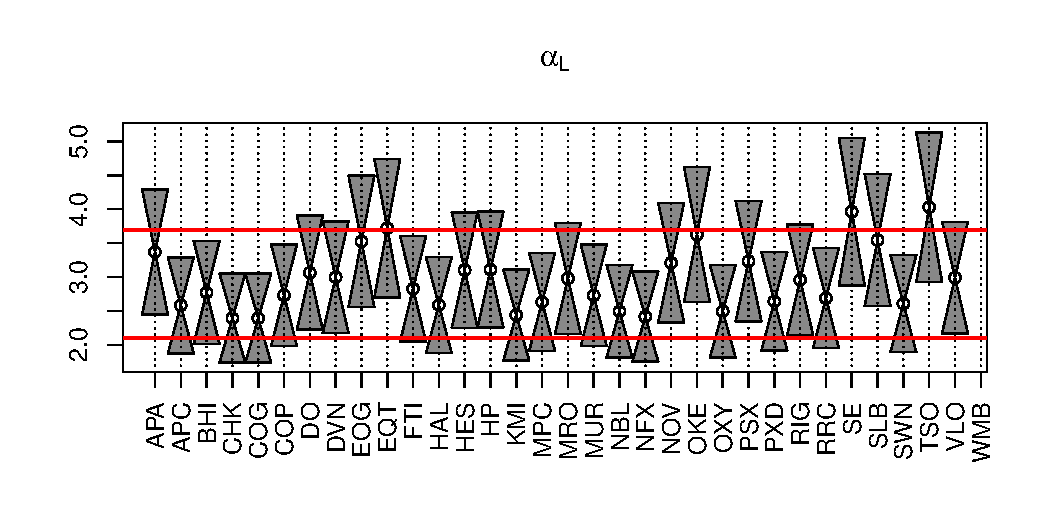
\includegraphics[width=\textwidth, trim={0, 0.8cm, 0, 2cm}, clip]
                        {Energy_lower.pdf}
      \end{minipage}
      \begin{minipage}{1.0\linewidth}
        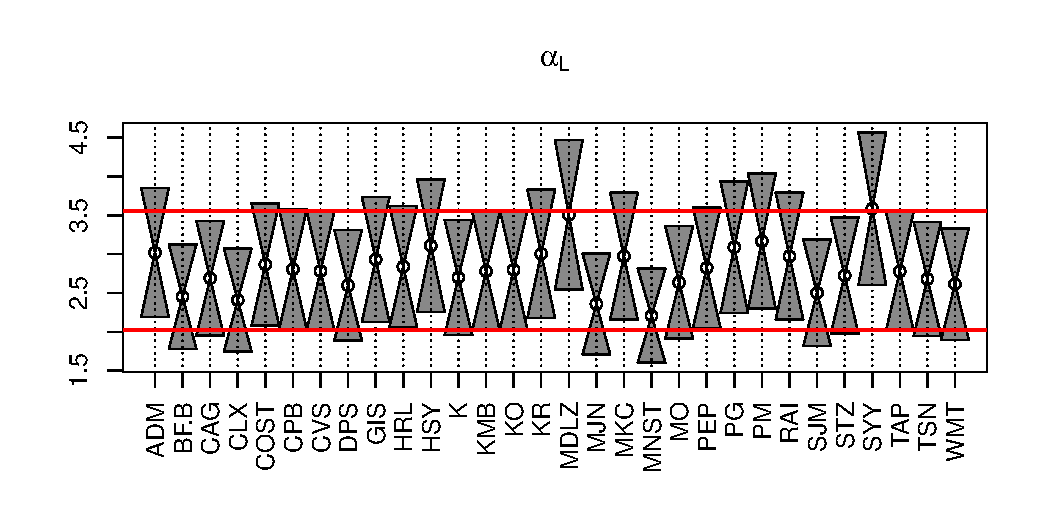
\includegraphics[width=\textwidth, trim={0, 0.8cm, 0, 2cm}, clip]
                        {Consumer_Staples_lower.pdf}
      \end{minipage}
      \begin{minipage}{1.0\linewidth}
        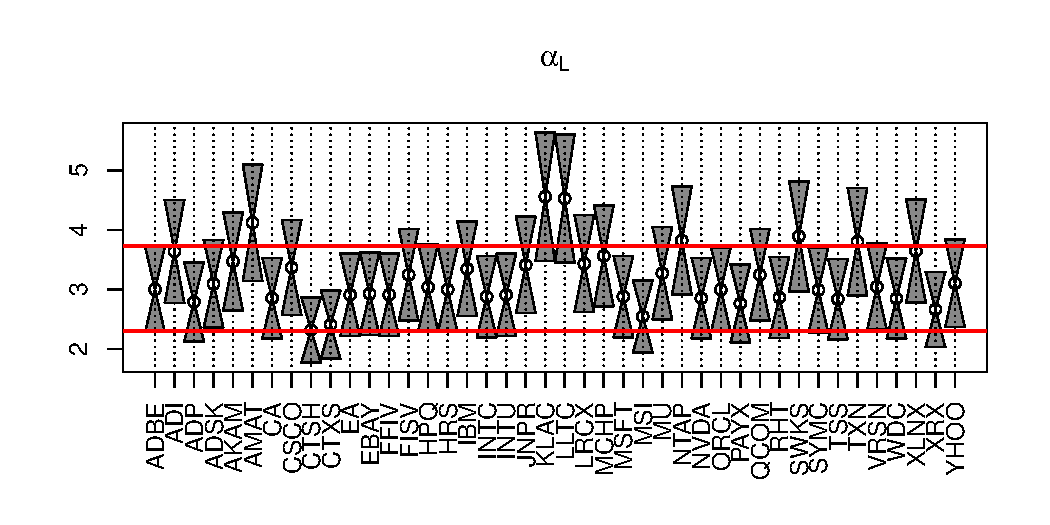
\includegraphics[width=\textwidth, trim={0, 0.8cm, 0, 2cm}, clip]
                        {Information_Technology_lower.pdf}
      \end{minipage}
      \caption{\tiny Hill estimates daily return series in
        sectors of the S\&P 500 index. The data span  from 1 January
        2010 to 31 December 2014 and comprise $n=1304$ observations.
        The graphs from top to bottom correspond to the {\bf ``Energy'',
        ``Consumer Staples'' and ``Information Technology''} sectors.
      }\label{fig:1}
    \end{figure}
  \end{minipage}\hfill
  \begin{minipage}[t]{0.5\linewidth}
    \textcolor[HTML]{990033}{\bf Interesting observations}
    \begin{itemize}
      \item Hill estimates of equity tail indices are often found
        between 2.5 $\sim$ 4.5
      \item The estimates are contained within each other's confidence bands
      \item Different sectors have different levels of variability in
        the tail indices.
    \end{itemize}
  \end{minipage}
\end{frame}

\begin{frame}
  \frametitle{Hill Estimator}
  Given a weakly dependent sequence $\{X_{i}\}_{i=1}^n$, the tail
  index($\alpha$) can be estimated using the Hill estimator
  \cite{embrechts:klueppelberg:mikosch:1997}:
  \[
  \hat \alpha = \left(
    {1 \over k} \sum_{i=1}^k \log{X_{(i)} \over X_{(k+1)}}
  \right)^{-1}
  \]
  where
  \begin{enumerate}
  \item $X_{(i)}$ is the $i$-th upper-order statistic of the sequence
  \item $k \to \infty$, $k/n \to 0$
  \end{enumerate}
  Moreover,
  \[
  \sqrt k (\hat \alpha - \alpha) \overset{d}{\to} N(0, \alpha^2)
  \]
\end{frame}

\begin{frame}
  \frametitle{Test for equal tail index: using Hill estimator}
  \begin{itemize}
    \item   Two return series $X_1, X_2, \dots, X_n$ and
      $Y_1, Y_2, \dots, Y_n$, with lower-tail indices
      $\alpha_X$ and $\alpha_Y$.
    \item We want to test the null hypothesis $H_0: \alpha_X = \alpha_Y$.
  \end{itemize}
  Under $H_0$, we have
  \[
  \sqrt k [\hat \alpha_X(k) - \hat \alpha_Y(k)] \overset{d}{\to}
  N(0, \alpha_X^2 + \alpha_Y^2)
  \]
  $\hat \alpha_X(k)$: Hill estimate of $\alpha_X$ using $k$ upper
  order statistics.
\end{frame}

\begin{frame}
  \frametitle{\small Test for equal tail index: testing for a
    changed extreme quantile}
  Given a series $X_1, X_2, \dots, X_n$ where $X_i \sim F_i$, Hoga
  \cite{hoga:2016} proposed a test for the hypothesis $H_0$:
  $1 < \exists k < n$ such that
  \begin{itemize}
    \item $F_i^{-1}(1 - p) = F_j^{-1}(1 - p)$, for all $1 \leq i < j < k$
    \item $F_{k-1}^{-1}(1 - p) \neq F_k^{-1}(1 - p)$ and
      $F_i^{-1}(1-p) = F_k^{-1}(1-p)$ for all $i \geq k$.
  \end{itemize}
  where $p = p_n \to 0$ as $n \to \infty$. The test statistic is
  \begin{tiny}
  \[
  T_n = \sup_{s \in [t_0, 1 - t_0]}
  \dfrac{  \big[s (1 - s) \log \big(\hat x_p(0, s)/\hat x_p(s, 1)\big)
      \big]^2}{
    \int_{t_0}^s\big[r \log \big( \hat x_p(0, r)/\hat x_p(0, s)
      \big)
      \big]^2 dr
    +
    \int_{s}^{1 - t_0}
    \big[
      (1 - r) \log \big(
      \hat x_p(r, 1)/
      \hat x_p(s, 1)
      \big)
      \big]^2 dr}
  \]
  \end{tiny}
  where
  \begin{small}
  \[
  \hat x_p(s, t) = X_{k, s, t}
  \left({n p \over k}\right)^{-1/{\hat \alpha}}
  \]
  \begin{itemize}
    \item $X_{k, s, t}$ is the $k$-th largest value among
      $X_{\floor{n s} + 1}, \dots, X_{\floor{n t}}$.
    \item The asymptotic distribution of $T_n$ under $H_0$ has to
      be Computed by simulation.
  \end{itemize}
  \end{small}
\end{frame}

\begin{frame}
  \frametitle{Results of the tests on S\&P 500 sectors}
\begin{figure}[htb!]
  \begin{minipage}{0.31\linewidth}
    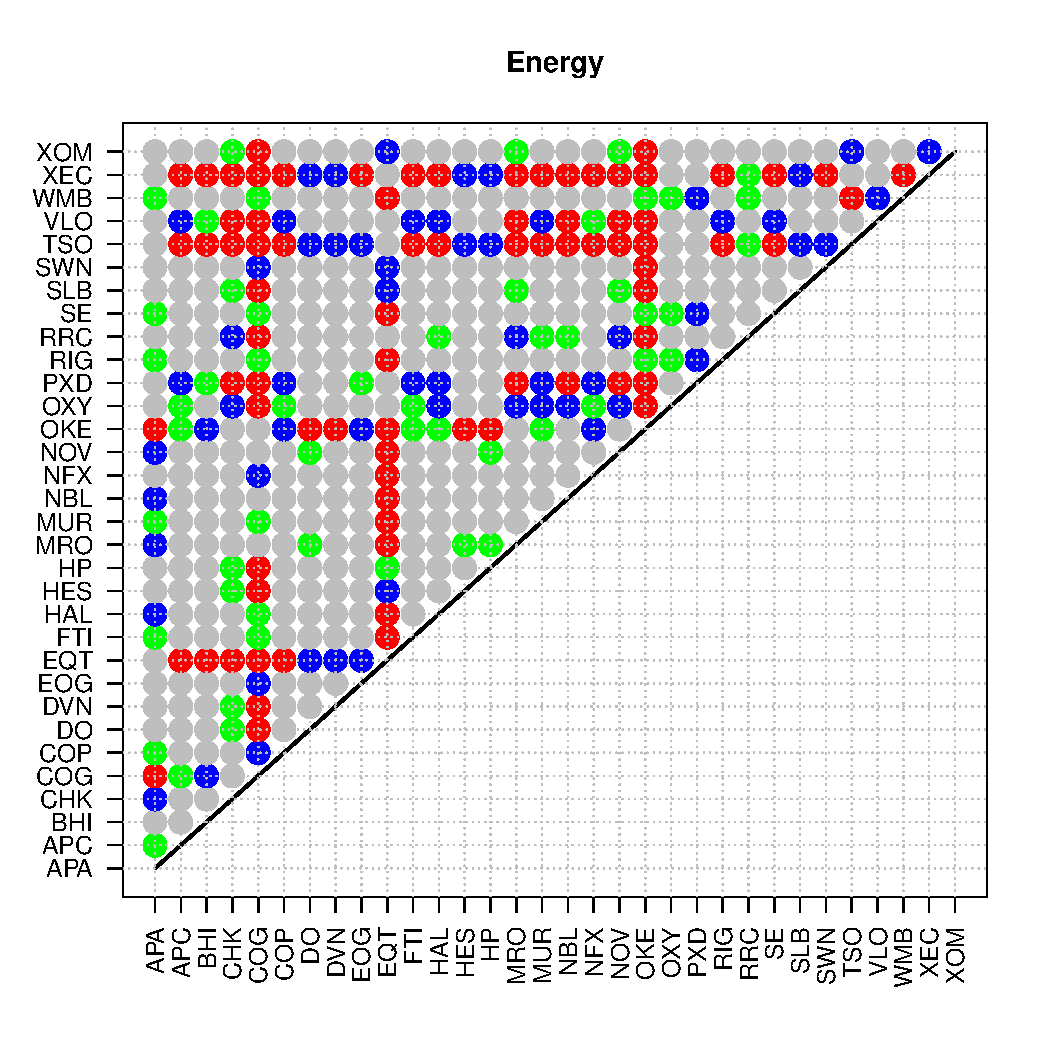
\includegraphics[
      width=\textwidth,
      trim={0.3cm, 0.8cm, 1cm, 0.6cm}, clip
    ]{HillTest_Energy.pdf}
  \end{minipage}\hfill
  \begin{minipage}{0.31\linewidth}
    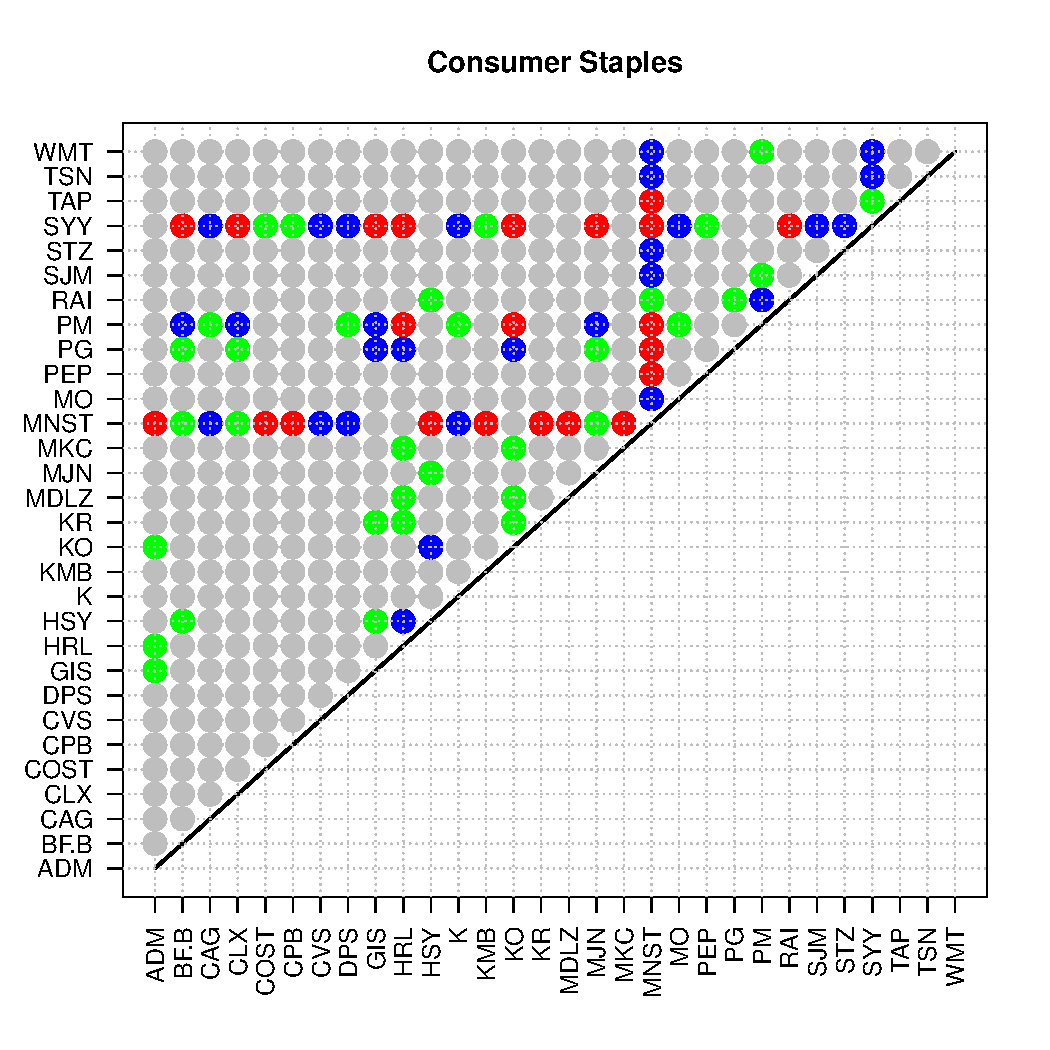
\includegraphics[
      width=\textwidth,
      trim={0.3cm, 0.8cm, 1cm, 0.6cm}, clip
    ]{HillTest_CS.pdf}
  \end{minipage}\hfill
  \begin{minipage}{0.31\linewidth}
    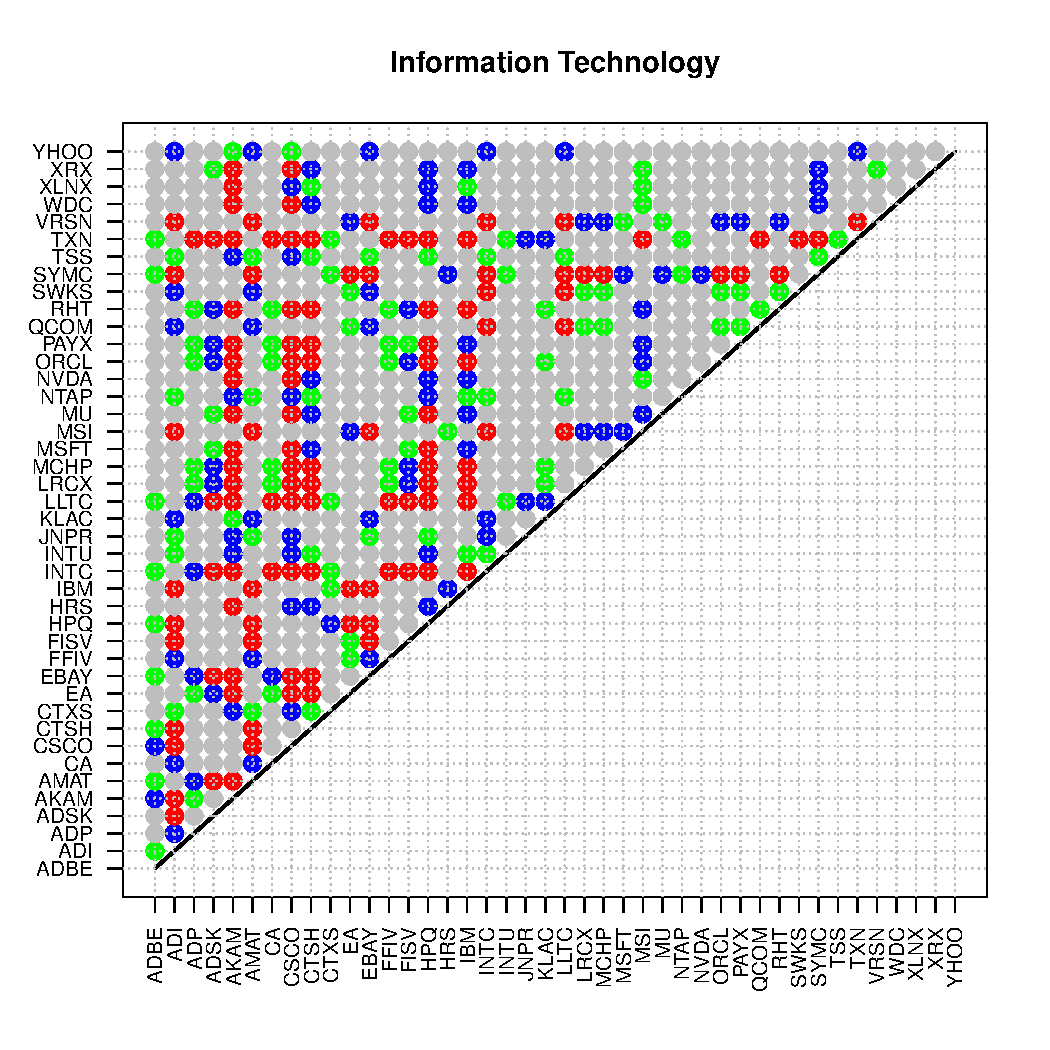
\includegraphics[
      width=\textwidth,
      trim={0.3cm, 0.8cm, 1cm, 0.6cm}, clip
    ]{HillTest_IT.pdf}
  \end{minipage}
  \begin{minipage}{0.31\linewidth}
    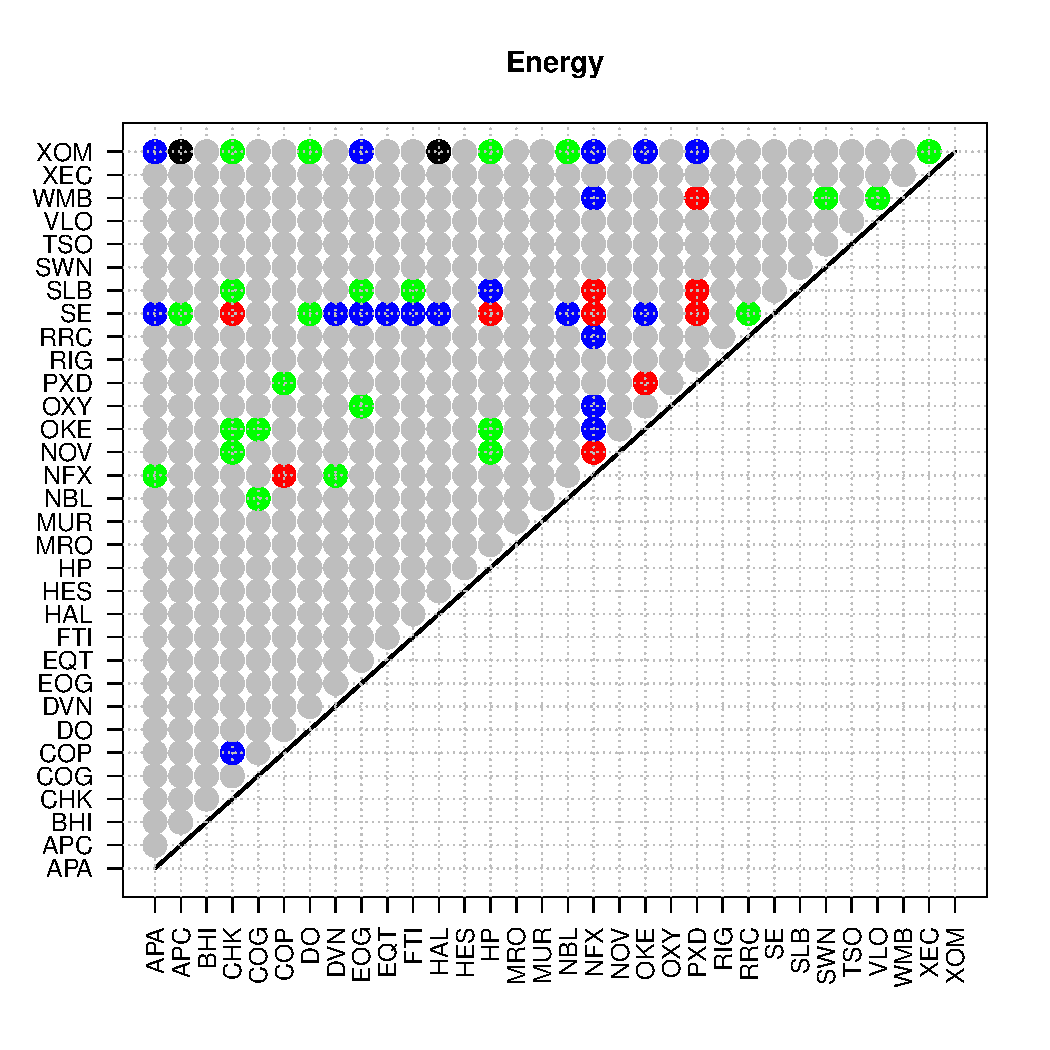
\includegraphics[
      width=\textwidth,
      trim={0.3cm, 0.8cm, 1cm, 0.6cm}, clip
    ]{Hoga_Energy_pair.pdf}
  \end{minipage}\hfill
  \begin{minipage}{0.31\linewidth}
    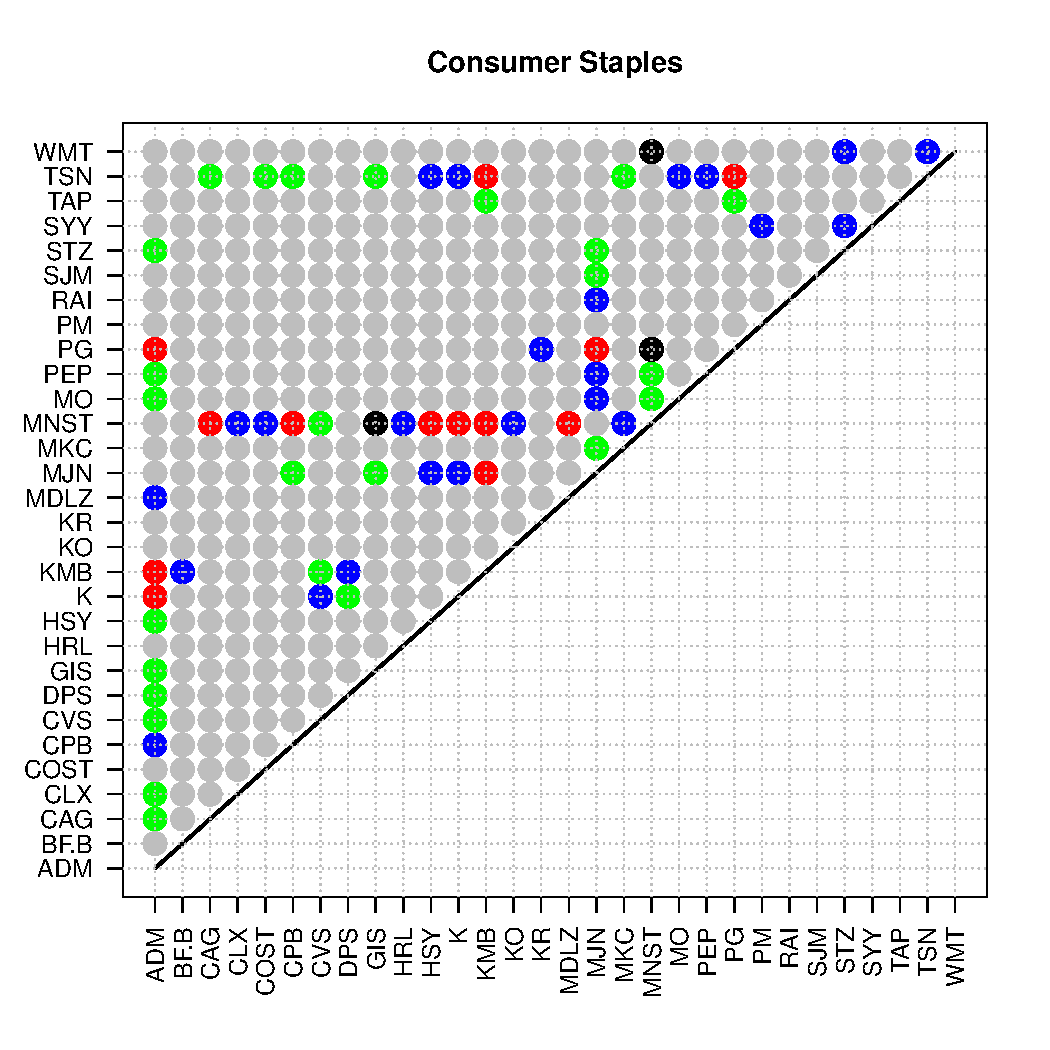
\includegraphics[
      width=\textwidth,
      trim={0.3cm, 0.8cm, 1cm, 0.6cm}, clip
    ]{Hoga_CS_pair.pdf}
  \end{minipage}\hfill
  \begin{minipage}{0.31\linewidth}
    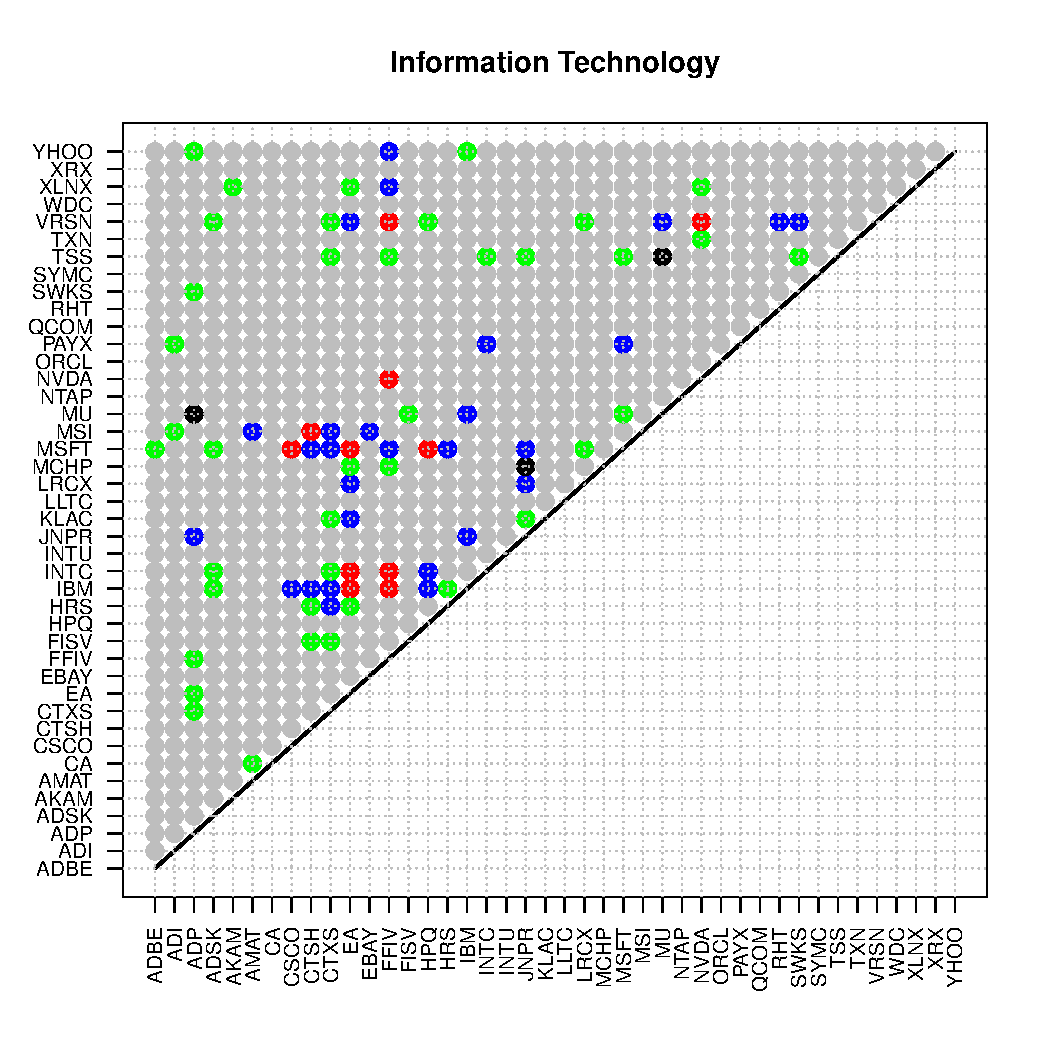
\includegraphics[
      width=\textwidth,
      trim={0.3cm, 0.8cm, 1cm, 0.6cm}, clip
    ]{Hoga_IT_pair.pdf}
  \end{minipage}
  \caption{\tiny
    {\em Top row}: Hill-based test.
    %% The test statistic in $\hat\alpha_X-\hat \alpha_Y$ is based
    %% on Hill estimates 
    %% of $\alpha_X$ and $\alpha_Y$. 
    The green, blue and red points correspond to pairs of stock in a sector
    when the test statistic is outside the intervals $[q_{0.075},q_{0.925}]$,
    $[q_{0.05},q_{0.95}]$,  $[q_{0.025},q_{0.975}]$
    %% $q_p$ is the $p$-quantile of the limiting 
    %% $N(0,\alpha_X^2+\alpha_Y^2)$-\ds\ of the test statistic in
    %% \eqref{eq:x1}. Grey points stand for pairs for which the test
    %% statistic is inside $[q_{0.075},q_{0.925}]$. 
    {\em Bottom row:} Hoga's test.
    The green, blue and red points correspond to pairs of stock in a sector 
    when the test statistic $T_n$ exceeds the $85\%$-, $90\%$-,
    $95\%$-quantile of the limit distribution .
  %% Grey points stand for pairs for which the test statistic is below
  %% the \asy\ $85\%$-quantile. Black points represent 
  %%   pairs for which the computation of $T_n$ fails for given precision  
  %%   requirements and time limits.
    The same number (50) of upper order statistics is used for both tests.}
  \label{fig:PairTest} 
\end{figure}
\end{frame}

\begin{frame}
  \frametitle{The scale parameter}
  Assume the equity return $X_t$ is stationary and follows Pareto
  distribution when $X < -K$:
  \[
  \P(X_t < -x) = {
    K^\alpha
    \over
    x^\alpha
  }, \quad x > K
  \]
  Hill's \cite{hill1975simple} maximum likelihood estimator for $K$ is
  \[
  \hat K_k = \left(
  {k \over n}
  \right)^{1/\hat \alpha_k} X_{(k)}
  \]
  where
  \begin{itemize}
  \item $n$ is the sample size
  \item $\hat \alpha_k$ is Hill's estimator of the tail index of $k$
    upper order statistics.
  \item $X_{(k)}$ is the $k$-th upper order statistic in the sample
  \end{itemize}
  By asymptotic normality of upper order statistics,
  \[
  \sqrt k (\hat K_k - K) \overset{d}{\to} N(0, K^2/\alpha^2)
  \]
\end{frame}

\begin{frame}
  \frametitle{Hill estimates of the scale parameter for S\&P 500
    sectors}
  {\scriptsize
  S\&P 500: Standard \& Poor's stock index. A weighted average of
  prices of 500 or so stocks listed on NYSE and NASDAQ. Stocks are
  grouped into 10 sectors. The \textcolor[HTML]{990033}{\bf Energy,
    Consumer Staples, IT} sectors are shown here.}
  \begin{minipage}{0.65\linewidth}
  \begin{figure}[htb!]
    \centering
    \begin{minipage}{0.33\linewidth}
      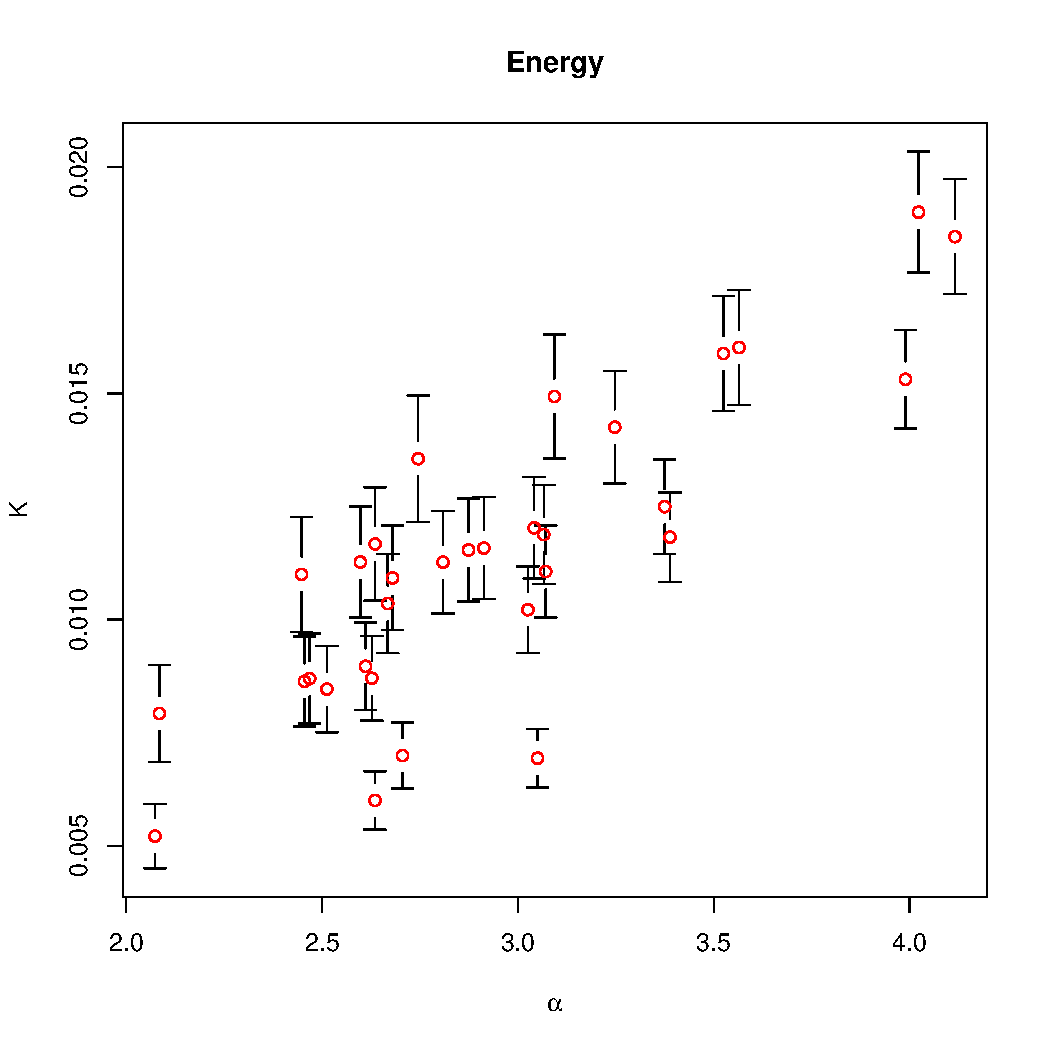
\includegraphics[width=\textwidth]
                      {Energy_K.pdf}
    \end{minipage}\hfill
    \begin{minipage}{0.33\linewidth}
      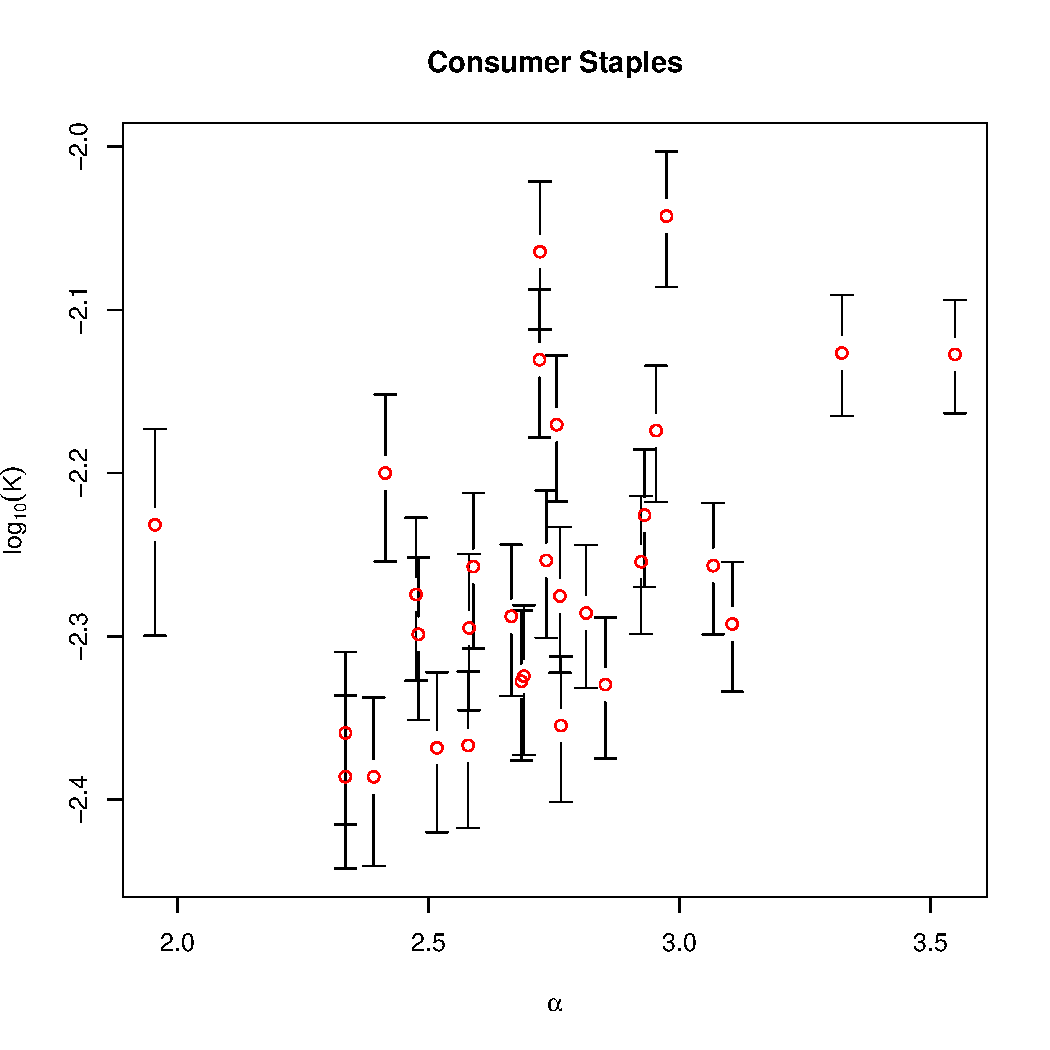
\includegraphics[width=\textwidth]
                      {CS_K.pdf}
    \end{minipage}\hfill
    \begin{minipage}{0.33\linewidth}
      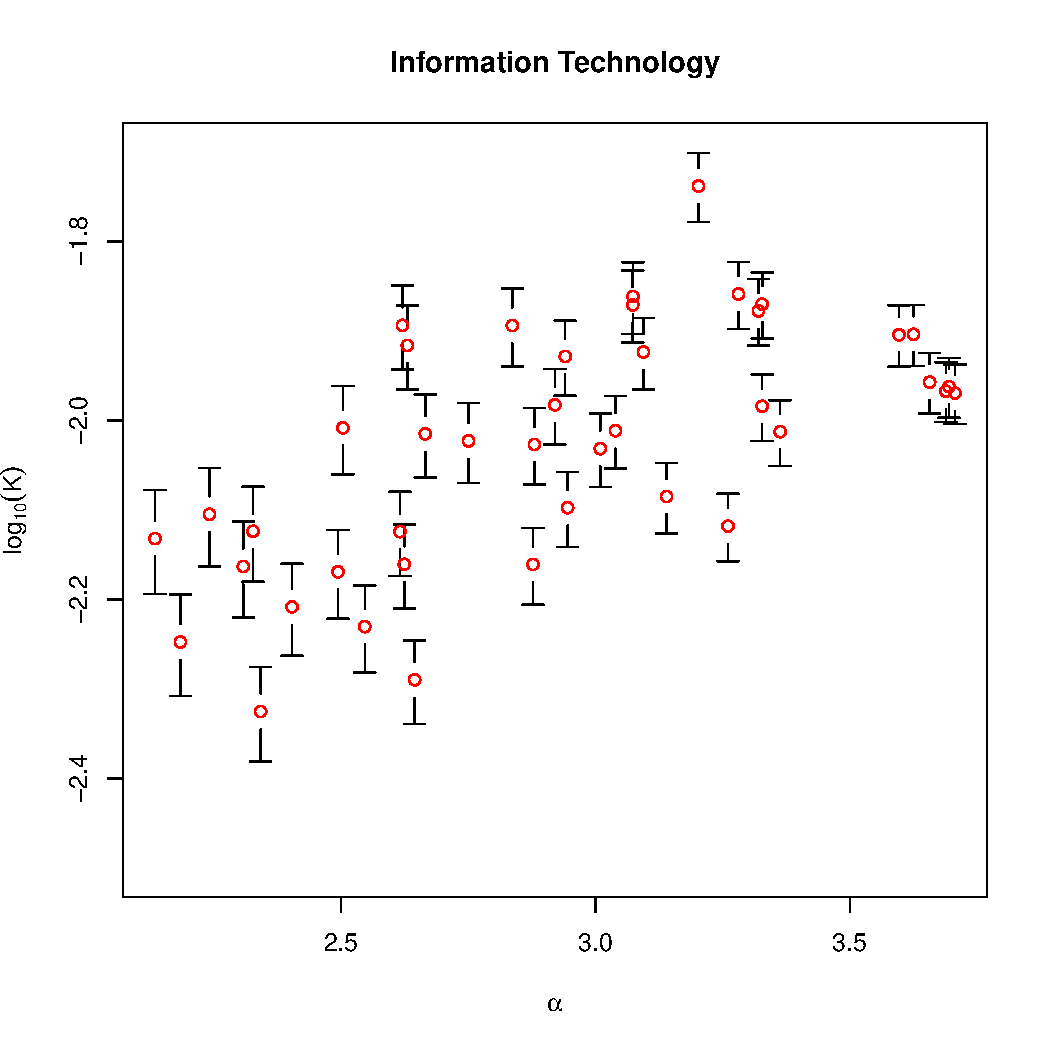
\includegraphics[width=\textwidth]
                      {IT_K.pdf}
    \end{minipage}
  \begin{minipage}{0.33\linewidth}
    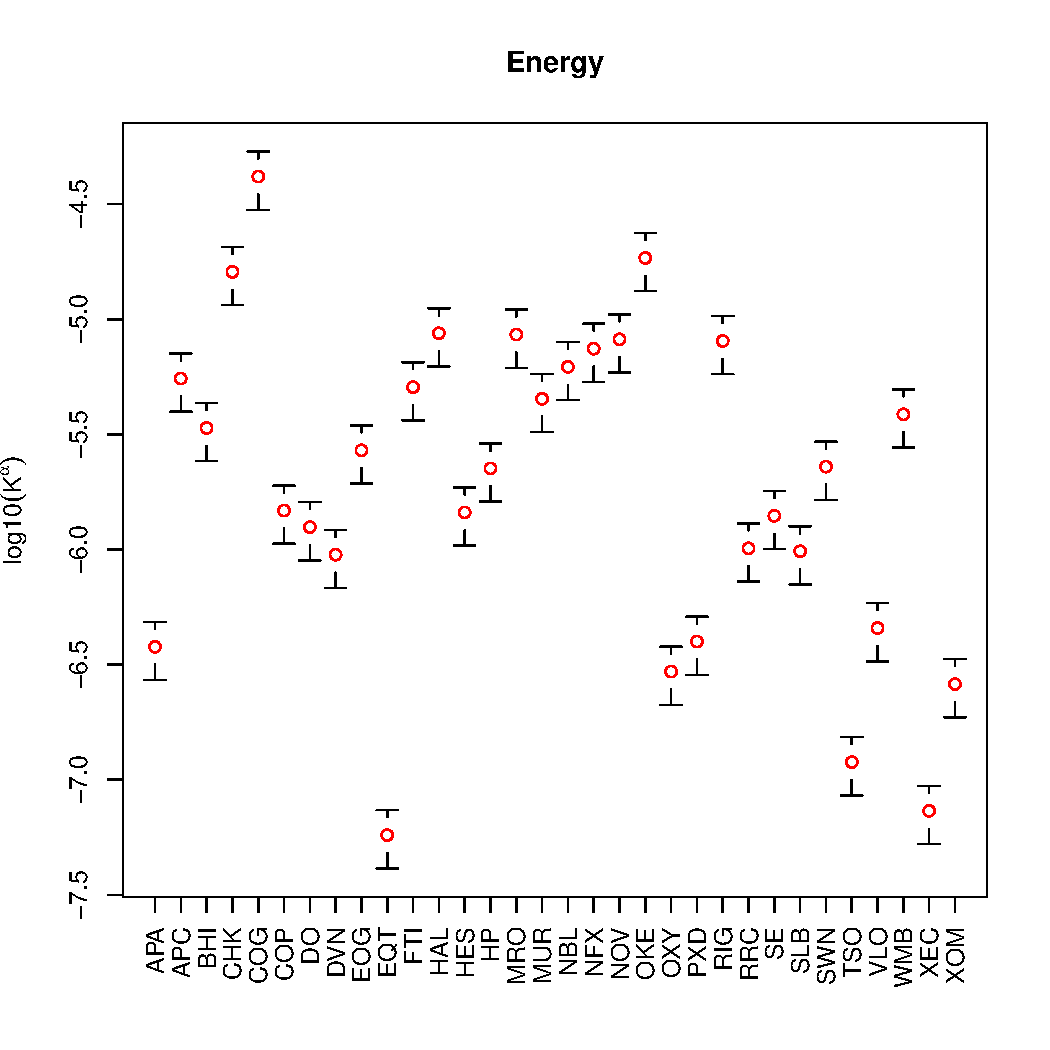
\includegraphics[width=\textwidth]
    {Energy_scale.pdf}
  \end{minipage}\hfill
  \begin{minipage}{0.33\linewidth}
    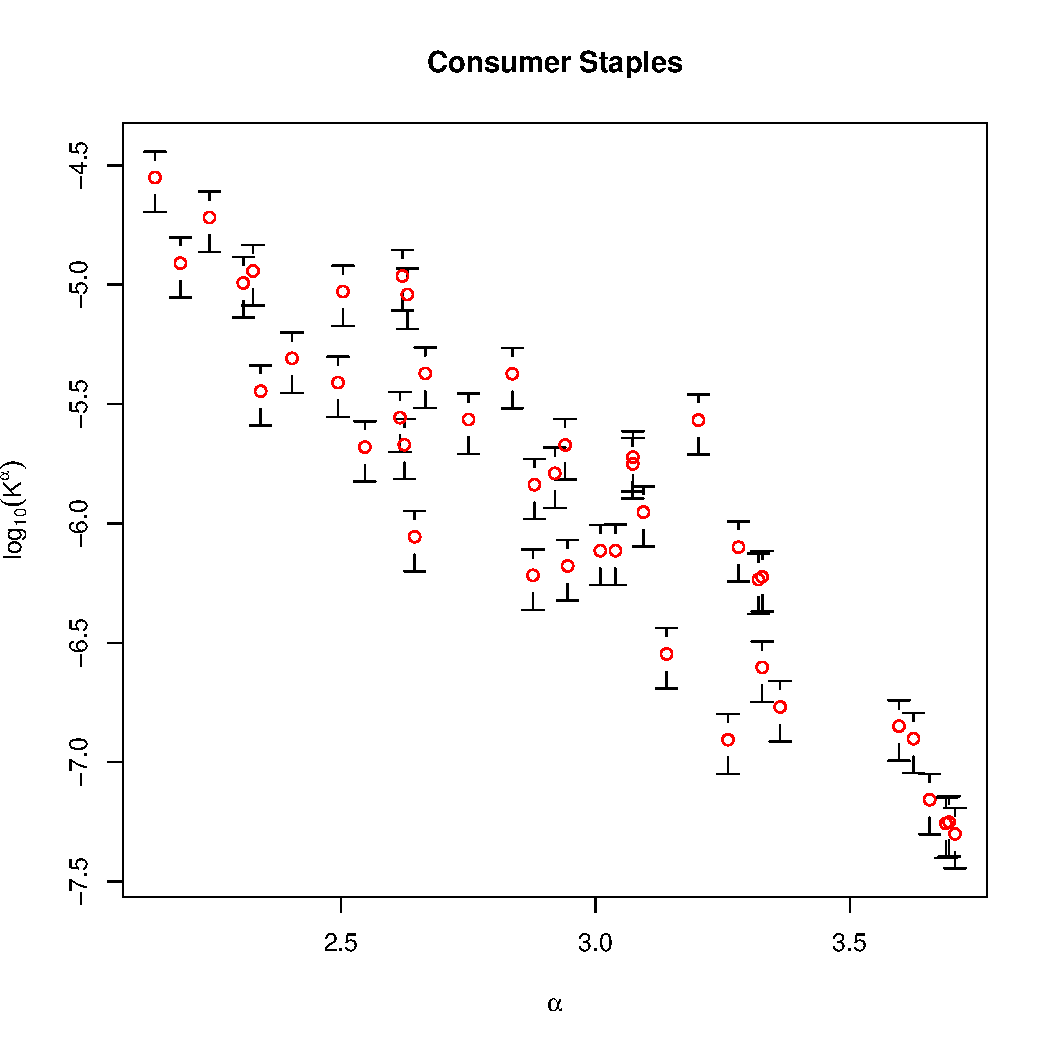
\includegraphics[width=\textwidth]
    {CS_scale.pdf}
  \end{minipage}\hfill
  \begin{minipage}{0.33\linewidth}
    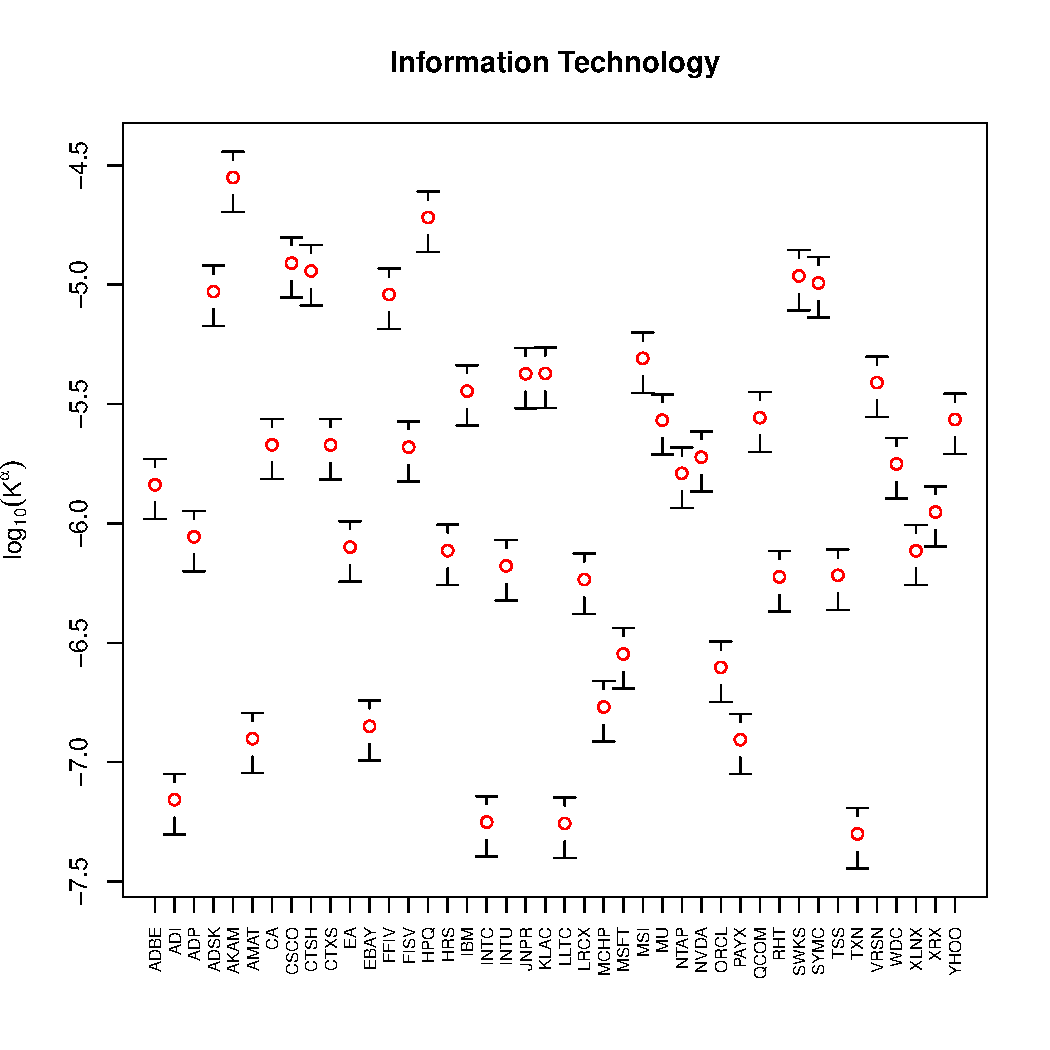
\includegraphics[width=\textwidth]
    {IT_scale.pdf}
  \end{minipage}
    \caption{\scriptsize Estimates of $\hat K_k$ (top) and
      $\hat K_k^{\hat \alpha}$ (bottom) on $\log_{10}$-scale.
      The bars are the asymptotic 95\%-confidence intervals.
    }
    \label{fig:sectors_parameters}
  \end{figure}
  \end{minipage}\hfill
  \begin{minipage}{0.35\linewidth}
    \begin{footnotesize}
      \begin{itemize}
      \item Estimated tail indices ($\hat \alpha$) and scale parameters
        $\hat K$ are positively dependent.
      \item The positive dependence is stronger for energy and IT stocks
        than for consumer staple's stocks.
      \item The scale $\hat K^{\hat \alpha}$ varies much more across different
        equities than does the tail index $\alpha$.
      \end{itemize}
    \end{footnotesize}
  \end{minipage}
\end{frame}

\begin{frame}
  \frametitle{Model of the market \& equity returns}
  \textcolor[HTML]{990033}{\bf The toy market consists of}
  \begin{enumerate}
  \item A riskless bond that pays $e^r$ kr. annually for each kr. invested,
    $r$ is fixed.
  \item A risky equity that pays $e^X$ kr. annually for each kr. invested.
    $X$ has Pareto tails
    \[
    F_X(x) = \left\{
      \begin{array}{ll}
        p \left(
          {K \over K - x}
        \right)^\alpha & x \leq 0 \,,\\
        1 - (1 - p) \left(
          {K' \over K' + x}
        \right)^\beta & x > 0\,,
      \end{array}
    \right.
    \]
  \end{enumerate}
\end{frame}

\begin{frame}
  \frametitle{Model of the investor}
  \begin{enumerate}
  \item He has 1 unit of currency for investment
  \item His happiness is proportional to a utility function $u(C)$:
    \begin{eqnarray*}
      C &=& (1 - \phi)e^r + \phi e^X \\
      u(C) &=& -C^{-\xi}/\xi, \quad \xi > 0 
    \end{eqnarray*}
    where
    \begin{itemize}
    \item $C$ is his monetary amount of consumption
    \item $\phi$ is the portion of his asset allocated to the equity
    \end{itemize}

  \item His preference over the equity is given by {\em
      Generalized Disappointment Aversion} \cite{routledge2010generalized}:
    \[
    \tilde u (F_X, \phi) = \E u(C) - b \E [u(v) - u(C); C < v]
    \]
    where
    \begin{itemize}
    \item $v$ is the level of consumption below which
      the investor will be disappointed
    \item $b$ captures how disappointed the investor will be in case his consumption
      falls below $v$.
    \end{itemize}
  \end{enumerate}
\end{frame}

\begin{frame}
  \frametitle{Analytic results: when $\alpha$ and  $\beta$ are independent}
  \begin{minipage}[t]{0.5\linewidth}
    \begin{figure}[htb!]
      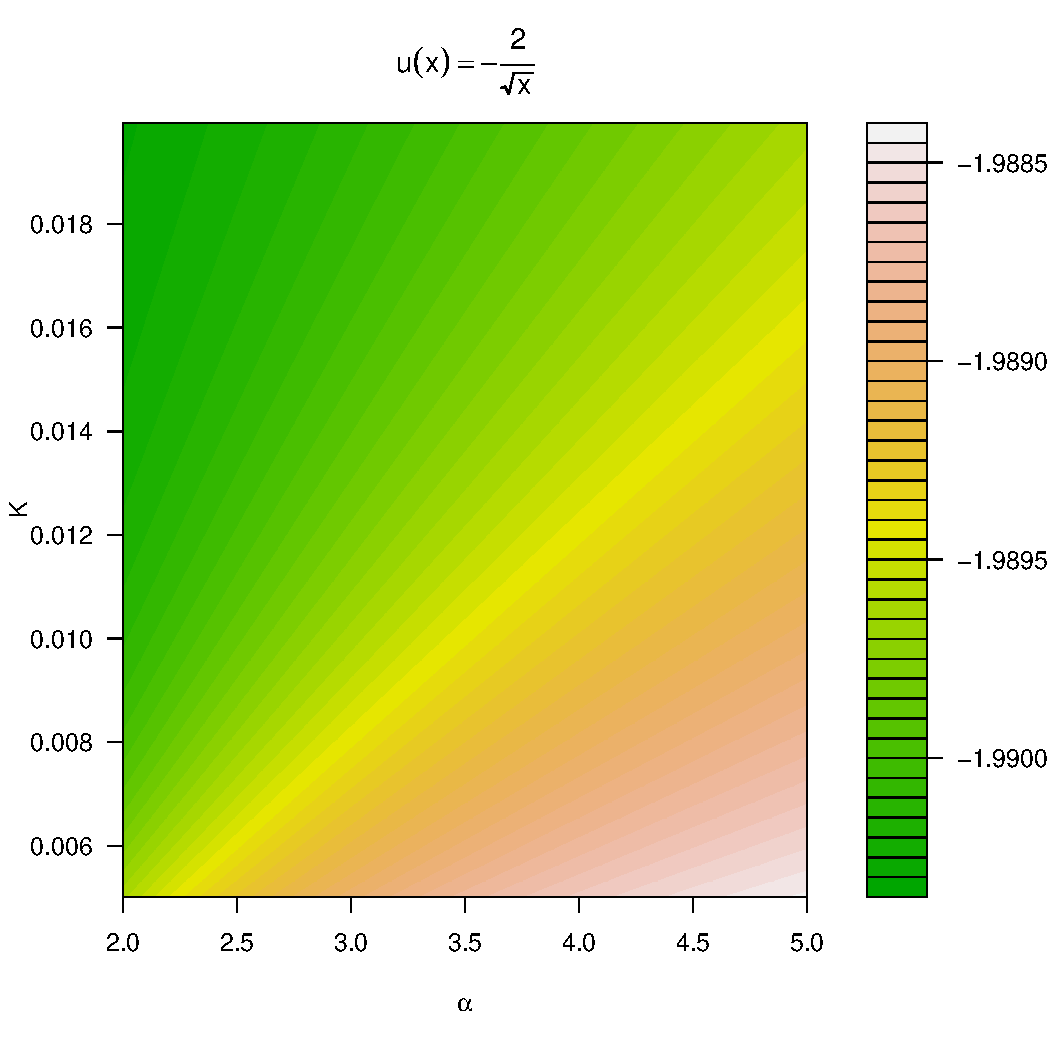
\includegraphics[width=\textwidth]{preference_pareto5e-1_A.pdf}
      \caption{\scriptsize
        $\tilde u_{\rm max}$ as a function of $\alpha$ and $K$
        in the two-sided Pareto model with $K'=0.012$, $\beta = 1.4$.
        $b = 0.01$ in all cases.
      }
    \end{figure}
  \end{minipage}\hfill
  \begin{minipage}[t]{0.5\linewidth}
    \begin{small}
      \begin{itemize}
      \item The investor's preference $\tilde u$ increases with $\alpha$ and
        decreases with $K$.
      \item Moving along a curve of equal preference, if $\alpha$
        increases then $K$ also increases.
      \item At market equilibrium, all actively traded stocks should
        have nearly the same investor preference -- $\alpha$ and
        $K$ values are expected to have positive dependence.
        % -- \textcolor[HTML]{990033}{\bf consistent with empirical results
        %   shown in figure \ref{fig:sectors_parameters}}.
        -- {\bf consistent with empirical results shown in figure
          \ref{fig:sectors_parameters}}.
      \end{itemize}
    \end{small}
  \end{minipage}
\end{frame}

\begin{frame}
  \frametitle{Analytic results: when $\alpha = \beta$}
  \begin{minipage}[t]{0.4\linewidth}
    \begin{figure}[htb!]
      \begin{minipage}{\linewidth}
        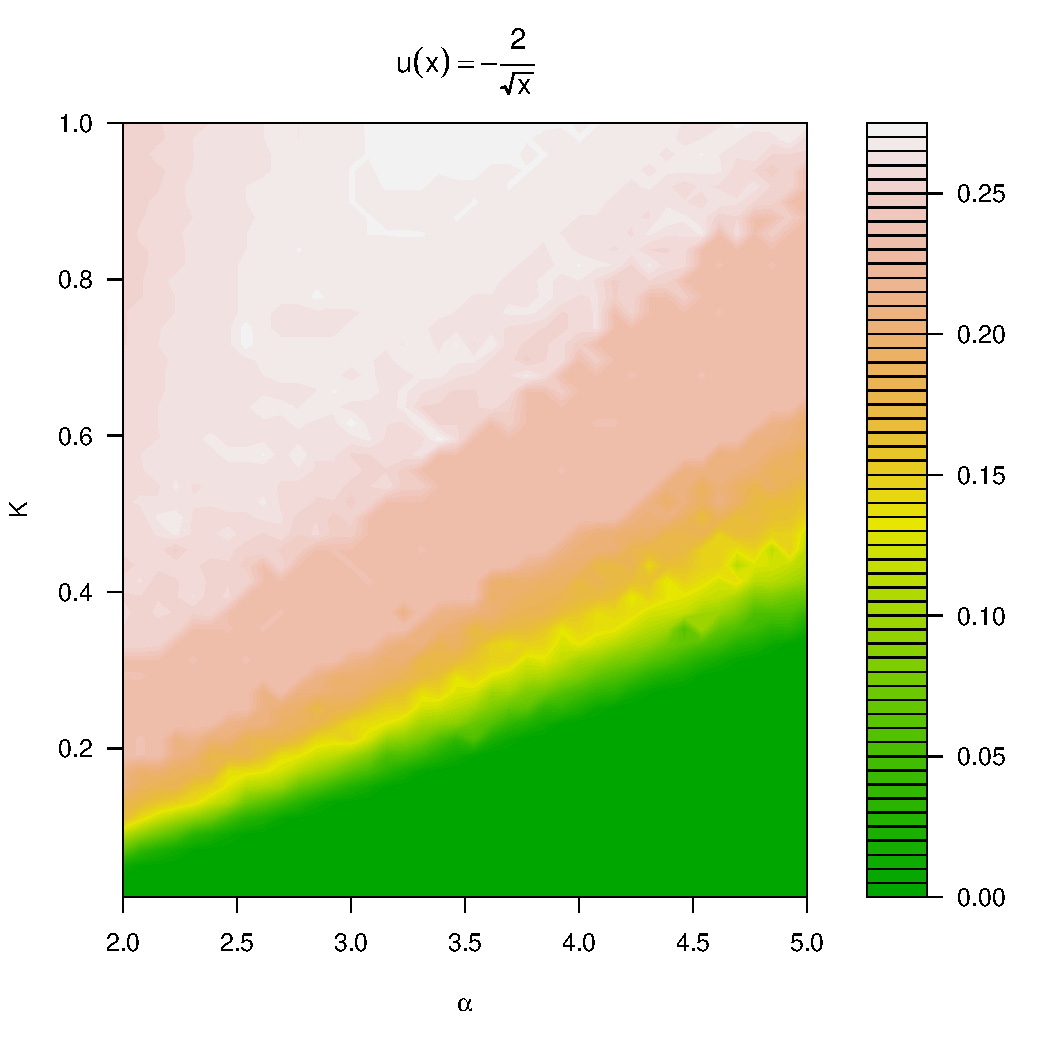
\includegraphics[width=1.0\textwidth, trim={0, 0, 0, 2cm}, clip]{phi_hat_pareto5e-1.pdf}    
      \end{minipage}\hfill
      \begin{minipage}{\linewidth}
        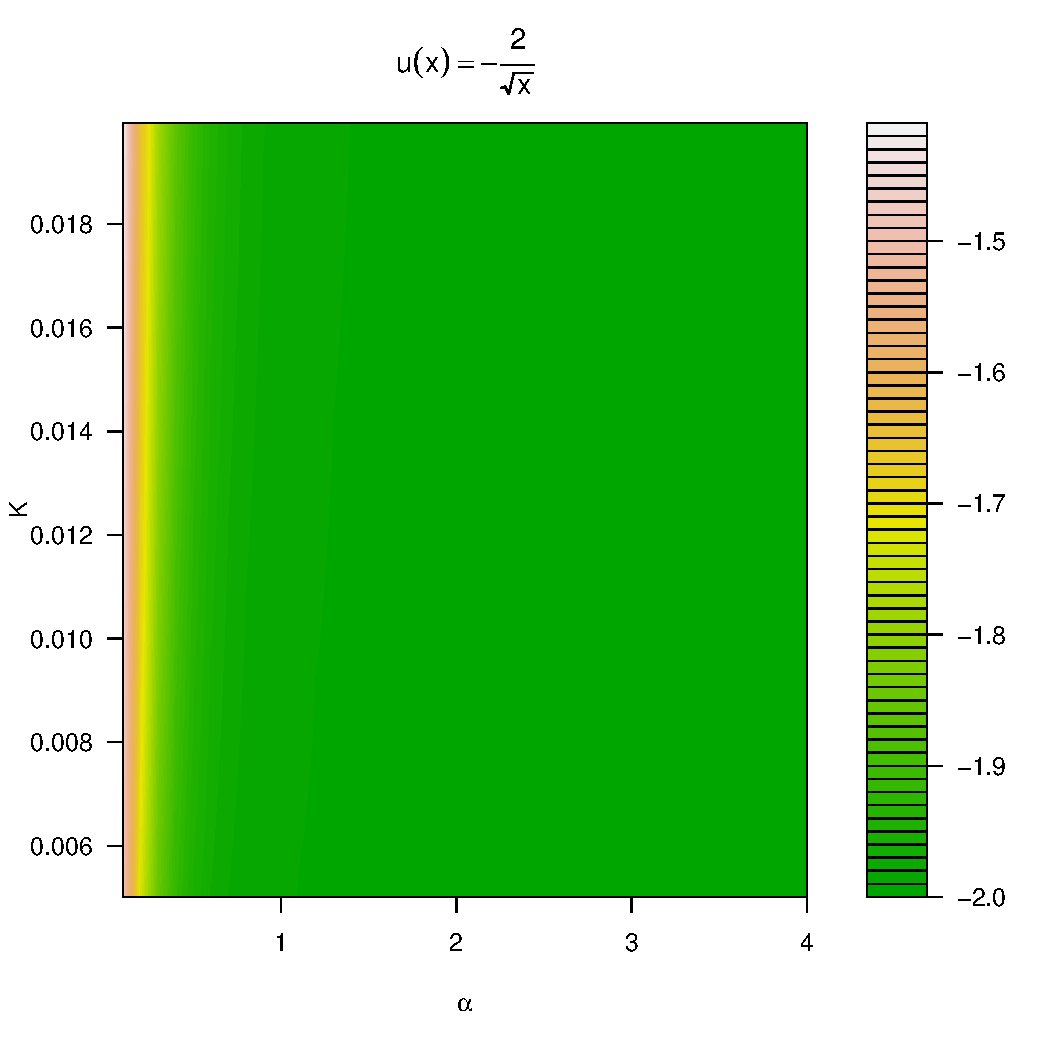
\includegraphics[width=1.0\textwidth, trim={0, 0, 0, 2cm}, clip]{preference_pareto5e-1.pdf}        
      \end{minipage}
    \end{figure}
  \end{minipage}\hfill
  \begin{minipage}[t]{0.6\linewidth}
    \begin{footnotesize}
      \textcolor[HTML]{990033}{\bf What's on the left?}
      \begin{itemize}
      \item Top: $\hat \phi(\alpha, K) = \argmax_{\phi} \tilde u(\alpha, K, \phi)$:
        optimal portion of allocation to the equity.
      \item Bottom: $\tilde u_{\rm max}(\alpha, K) = \max_{\phi} \tilde
        u(\alpha, K, \phi)$:
        Investor preference with optimal equity allocation.
      \item utility function $u(x) = -\frac{2}{\sqrt x}$
      \end{itemize}
      
      \textcolor[HTML]{990033}{\bf What I see from the plots}
      \begin{itemize}
      \item $\hat \phi$ is not monotone w.r.t. $\alpha$ or $K$.
      \item For a fixed $K$, $\hat \phi$ is decreasing with $\alpha$
        when $\alpha$ is in the range 2.5 $\sim$ 4.5, typical for real
        equity return series.
      \item $\tilde u_{\rm max}(\alpha, K)$ decreases with $\alpha$ 
        but is rather insensitive to $K$.
      \end{itemize}
    \end{footnotesize}
  \end{minipage}
\end{frame}

\begin{frame}
  \frametitle{When equity returns have t-distribution \& $b = 0$}
  The GDA preference reduces to {\em expected utility}. A few cases
  arise depending on
  \[
  a = {
    (1 - \phi) e^r
    \over
    \phi
  }, \quad
  y_\pm = {
    a^2 - \xi \pm \sqrt{(a^2 - 1) (a^2 - \xi^2)}
    \over
    a (\xi - 1)
  }
  \]
\begin{enumerate}
\item If $\max\{a, 1\} < \xi$, $\tilde u_{\rm max}$ is
  monotone increasing with $\alpha$.
\item If $a < \xi < 1$ and $(a + y_-)/(a y_- + 1) <
  y_-^{(1-\xi)/(1+\xi)}$, $\tilde u_{\rm max}$ is monotone
  increasing with $\alpha$.
\item If $\xi < a < 1$, $\tilde u_{\rm max}$ is monotone
  decreasing with $\alpha$.
\item If $1 < \xi < a$ and $(a + y_+)/(a y_+ + 1) >
  y_+^{(1-\xi)/(1+\xi)}$, $\tilde u_{\rm max}$ is monotone
  decreasing with $\alpha$.
\item In other case, $\tilde u_{\rm max}$ is not monotone
  w.r.t. $\alpha$.
\end{enumerate}
\end{frame}

\begin{frame}
  \frametitle{When equity returns have t-distribution \& $b > 0$}
  \begin{minipage}[t]{0.5\linewidth}
    \begin{figure}[htb!]
      \begin{minipage}{0.5\linewidth}
        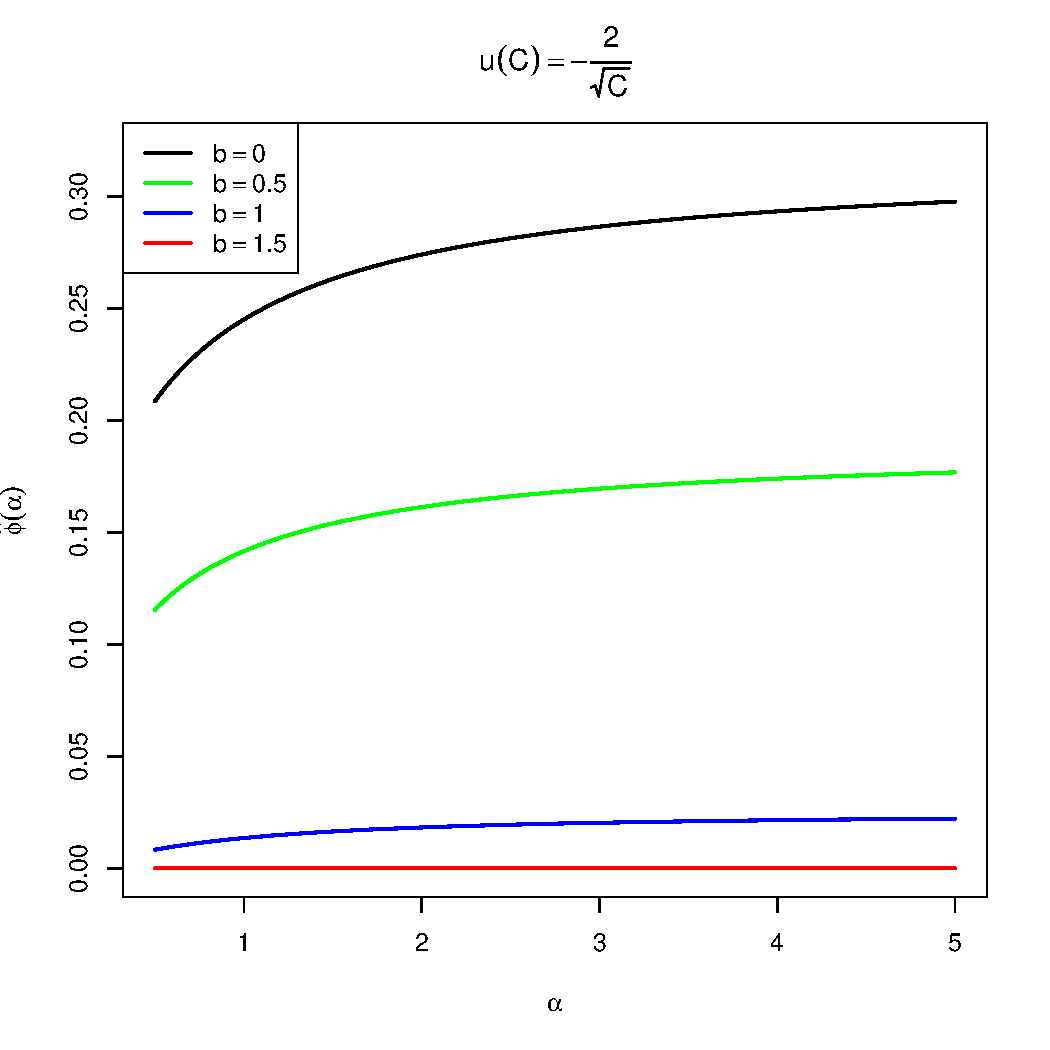
\includegraphics[width=\textwidth]{phi_hat_b_t_power.pdf}
      \end{minipage}\hfill
      \begin{minipage}{0.5\linewidth}
        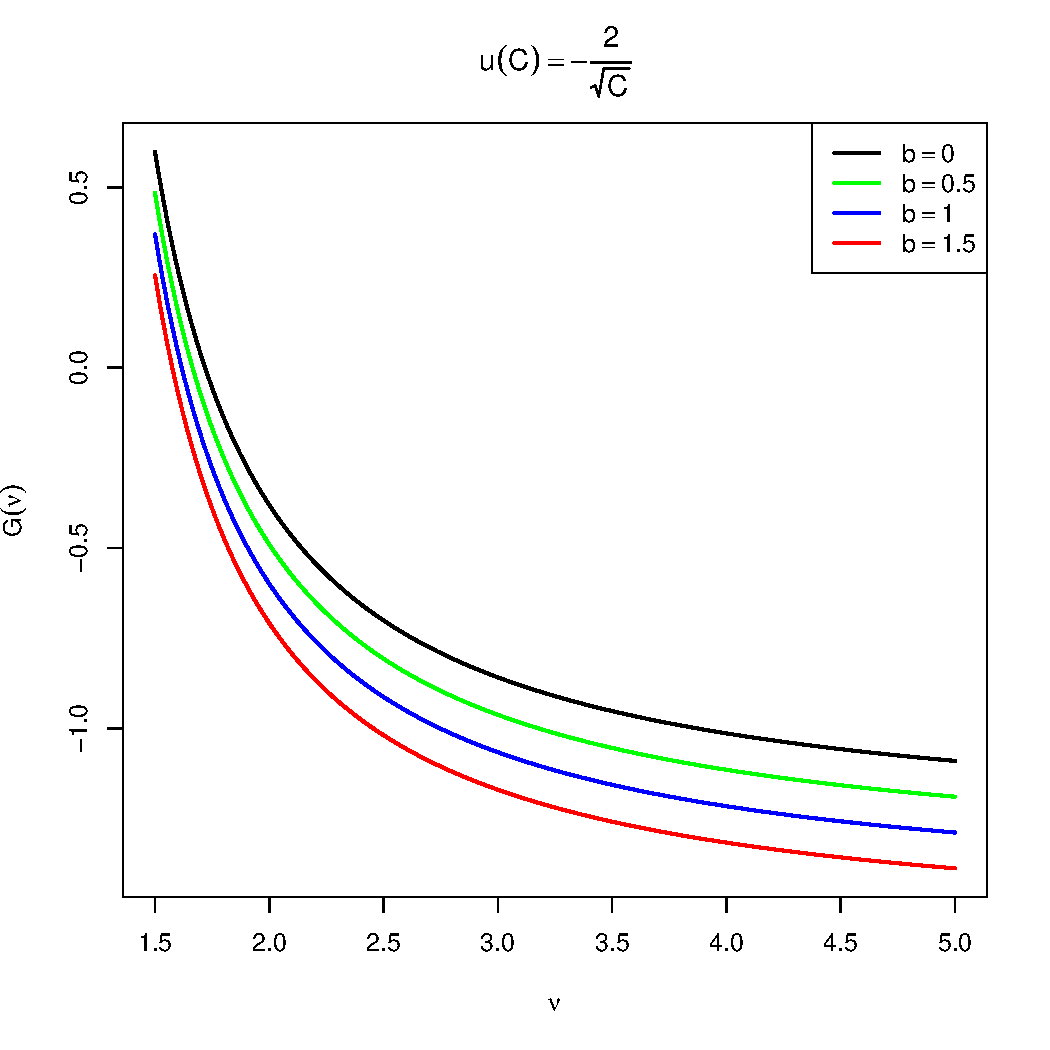
\includegraphics[width=\textwidth]{U_b_t_power.pdf}
      \end{minipage}
      \begin{minipage}{0.5\linewidth}
        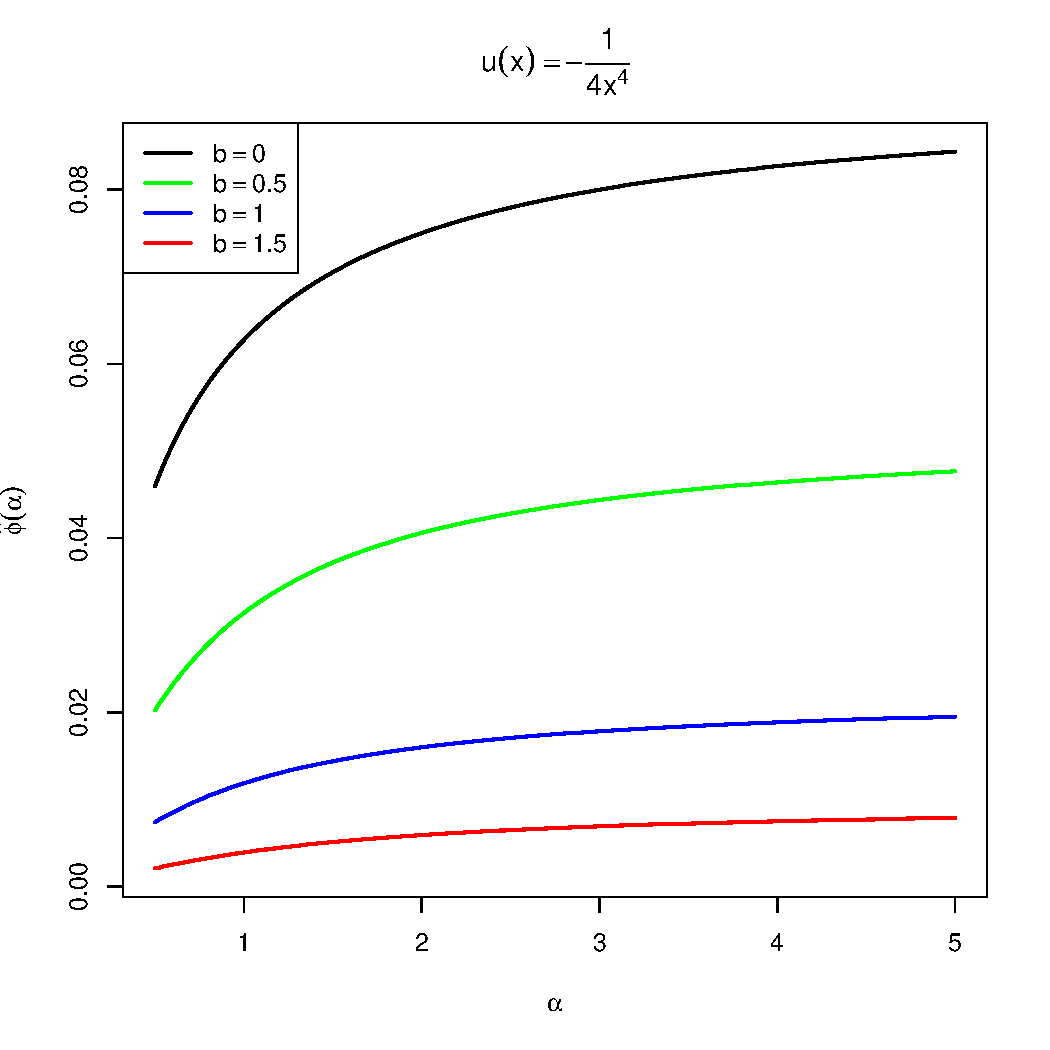
\includegraphics[width=\textwidth]{phi_hat_b_t_power4.pdf}
      \end{minipage}\hfill
      \begin{minipage}{0.5\linewidth}
        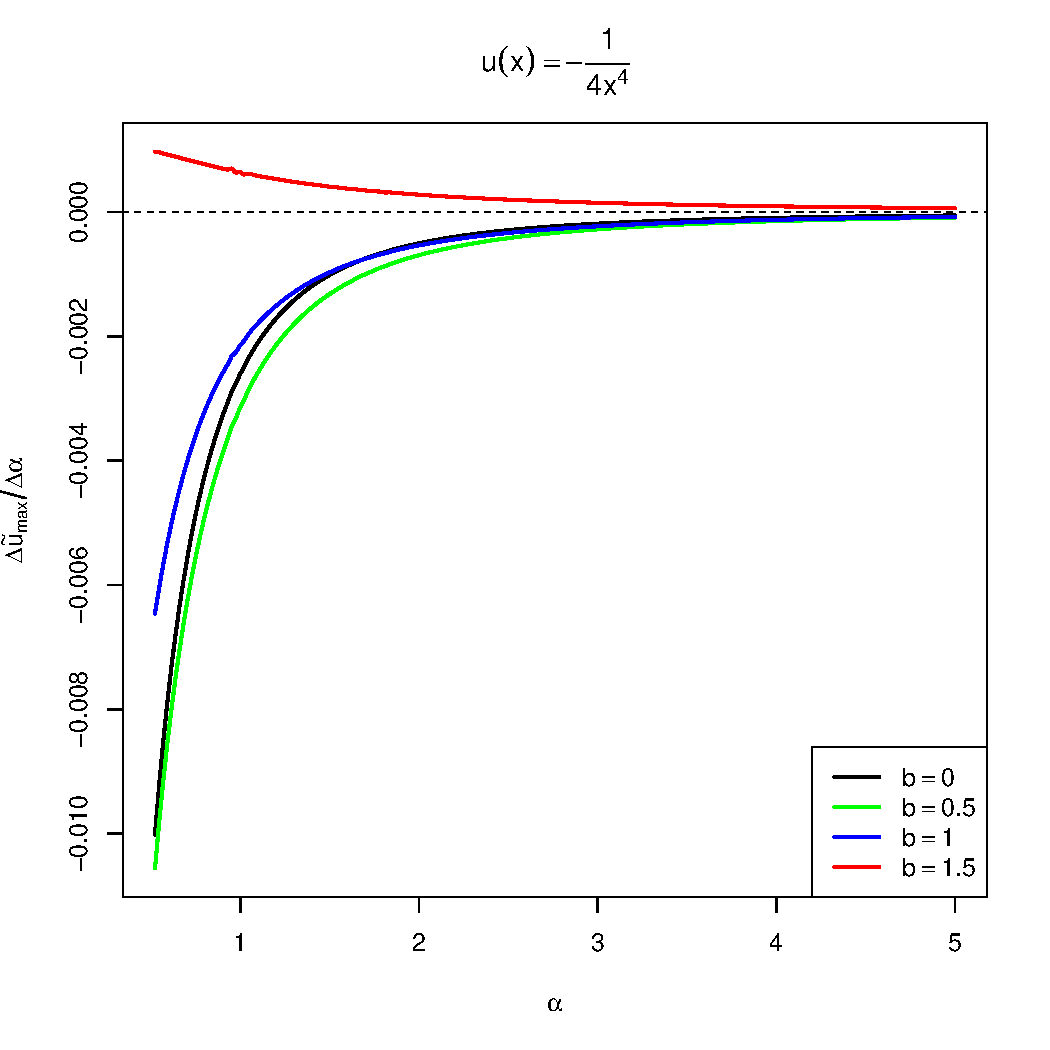
\includegraphics[width=\textwidth]{U_b_t_power4.pdf}
      \end{minipage}
      \caption{$\hat\phi$ (left) and
        ${\partial \tilde u_{\rm max} \over \partial \alpha}$ (right).
        {\em top:} $\xi = 1/2$. {\em bottom:} $\xi = 4$.
      }
      \label{fig:htfg}
    \end{figure}
  \end{minipage}\hfill
  \begin{minipage}[t]{0.5\linewidth}
    \textcolor[HTML]{990033}{\bf The figure says:}
    \begin{itemize}
    \item  $\hat\phi$ is monotone increasing for all 4 values of $b$
    \item $\tilde u_{\rm max}(\alpha)$ is increasing with $\alpha$
      when $b$ is relatively large, but  decreasing with $\alpha$ when
      $b$ is small
    \item A sizable value of $b$ indicates a conservative, risk-averse investor.
    \end{itemize}
  \end{minipage}
\end{frame}

\begin{frame}
  \frametitle{Summary}
  \begin{itemize}
  \item The tail index varies to different extent in different
    sectors/markets.
  \item The scale parameter is positively dependent on the tail index.
  \item The scale $K^{\alpha}$ varies much more across different
    equities than does the tail index $\alpha$.
  \item An investor's preference over $\alpha$ is dependent on the
    riskless rate of return, his own utility function and how
    disappointed he will be if his investment falls below
    expectation.
  \end{itemize}
\end{frame}

%% \section{Rare event simulation for GARCH(p,q) processes}
\section{GARCH($p, q$) Importance Sampling}
\begin{frame}
  Rare event simulation for GARCH(p,q) processes
\end{frame}

\begin{frame}
  \frametitle{Importance Sampling Estimator}
  \underline{\scriptsize{
      Want to estimate $\P(X \in S) = \E \I_S(X)$:}
  }

  \begin{minipage}[t]{0.45\linewidth}
    \textcolor[HTML]{990033}{Naive Monte Carlo}
    \begin{small}
      \begin{eqnarray*}
        \E \1{X > u} &=& \int \1{X > u} f(x) dx
      \end{eqnarray*}
      Draw $n$ iid samples of $X$ from $f(x)$, say $x_1, ..., x_n$,
      then estimate $\P(X > u)$ as
      \[
      {1 \over n} \sum_{i=1}^n \I_S(X)
      \]
    \end{small}
  \end{minipage}\hfill
  \begin{minipage}[t]{0.5\linewidth}
    \textcolor[HTML]{990033}{Importance Sampling}
    \begin{scriptsize}
    \begin{itemize}
    \item Note
      \[
      \P(X > u)
      =
      \E^{\tilde \nu} \left[
        \underbrace{
          \td{\nu}{\tilde \nu}(X) \1{X > u}
        }_{\mathcal E_u}
      \right]
      \]
      where $\nu$ denotes the original prob. measure while $\tilde \nu$
      denotes the shifted prob. measure. $\td{\nu}{\tilde \nu}$ is the
      Radon-Nikodym derivative.
    \item A desirable choice of $\tilde \nu$:
      Choose the $\tilde \nu$ such that the {\em relative error}
      is bounded. Let $\P(X > u) \to 0,\; u \to \infty$. Choose
      $\tilde \nu$ such that
      \[
      \lim_{u \to \infty} {\var({\mathcal E}_u) \over \P(X > u)^2} < \infty
      \]
    \end{itemize}
    \end{scriptsize}
    % \begin{tiny}
    %   \begin{eqnarray*}
    %     \E \1{X > u} &=& \int \lambda(\alpha)\1{X > u} e^{-\alpha x}
    %                      {e^{\alpha x} f(x) \over \lambda(\alpha)} dx
    %   \end{eqnarray*}
    %   where
    %   \[
    %   \lambda(\alpha) = \int e^{\alpha x} f(x) dx < \infty
    %   \]
    %   So
    %   \[
    %   f_\alpha(x) = \frac{e^{\alpha x} f(x)}{\lambda(\alpha)}
    %   \]
    %   is a density function. Draw $x_1, ..., x_n$ from
    %   $f_\alpha(x)$ and estimate $\P(X > u)$ as
    %   \[
    %   {1\over n}\sum_{i=1}^n \lambda(\alpha) \1{x_i > u} e^{-\alpha x_i}
    %   \]
    %   \bf{One can show $\alpha$ for which
    %     $\lambda(\alpha) = 1$ minimises the relative error of the
    %     estmator.}
    % \end{tiny}
  \end{minipage}
\end{frame}

\begin{frame}
  \frametitle{GARCH(1,1) Probability of Large Exceedance}
    Want to estimate $\P(\sigma_t^2 > u)$ for large $u$. $\sigma_t^2
  \sim \pi$, the stationary distribution of $\sigma_t^2$.
  \begin{eqnarray*}
    \sigma_t^2
    &=&
    \alpha_1 X_{t-1}^2 + \beta_1 \sigma_{t-1}^2 + \omega \\
    &=&
    \underbrace{
      (\alpha_1 Z_{t-1}^2 + \beta_1)
    }_{A_t}  \sigma_{t-1}^2 + \omega
  \end{eqnarray*}
  It can be shown
   \[
   \P(\sigma^2_t > u) = {
     \E_\gamma N_u
     \over
     \E_\gamma K
   }
   \]
   where
   \begin{footnotesize}
     \begin{itemize}
     \item $K$ is the first time $\{\sigma_t^2\}$ returns to
       $\mathcal C = [0, M]$.
     \item $\sigma_0^2 \sim \gamma$,
       $\gamma(E) = \pi(E) / \pi(\mathcal C)$, for all
       $E \subseteq \mathcal C$.
     \item
       \[
       N_u = \sum_{i=0}^{K - 1} \1{\sigma^2_i > u}
       \]
     \item $\E_\gamma$: Start the process with
       $\sigma_0^2 \sim \gamma$. (cf.  Collamore and
       Vidyashankar \cite{Collamore20133378}).
     \end{itemize}
   \end{footnotesize}
 \end{frame}

%  \begin{frame}
%    \frametitle{GARCH(1,1) Probability of Large Exceedance}
%    Define
%    \begin{itemize}
%    \item $K_i$: the time when $\{V_t\}$ visits $\mathcal C$ for the
%      $i$-th time;
%    \item $\mathcal R_n$: Number of times that $\{V_t\}$ visits $\mathcal C$
%      before time $n$.
%    \end{itemize}
%    By law of large numbers for Markov chains (LLN):
%    \[
%      {1 \over m} \sum_{t=0}^{K_m - 1} \1{V_t > 0}
%      =
%      {1 \over m} \sum_{i=1}^m
%      \sum_{t=K_{i-1}}^{K_i - 1} \1{V_t > u}
%      \overset{a.s.}{\to}
%      \E_\gamma N_u     
%    \]
%    Also by LLN,
%    \[
%      {1 \over n} \sum_{t=0}^n \1{\sigma_t^2 > u}
%      \overset{a.s.}{\to}
%      \P(\sigma_t^2 > u)
%      \]
%      Meanwhile
%    \begin{eqnarray*}
%      {1 \over n} \sum_{t=0}^n \1{\sigma_t^2 > u}
%      &=&
%      {1 \over n}
%      \left[
%        \sum_{t=0}^{K_{\mathcal R_n} - 1} \1{\sigma_t^2 > u}
%        +
%        \sum_{t=K_{\mathcal R_n}}^{n} \1{\sigma_t^2 > u}
%      \right]
%    \end{eqnarray*}
%  \end{frame}

\begin{frame}
  \frametitle{GARCH(1,1) Probability of Large Exceedance}
  It can be shown
  \[
  \P(\sigma_t^2 > u) = \pi(\mathcal C) \E_\gamma (N_u)
  \]
  \begin{itemize}
  \item find an unbiased importance sampling estimator $\mathcal E_u$ for
     $\E_\gamma (N_u)$, then $\pi(\mathcal C) \mathcal E_u$ is an unbiased estimator
     for $\P(\sigma_t^2 > u)$.
   \item $\pi(\mathcal C)$ also needs to be estimated, but this can be done with the original measure.
   \item Our importance sampling estimator $\mathcal E_u$
     \[
     \E_\gamma(N_u) = \E_\gamma^{\mathcal D} \left[
       \underbrace{
         e^{-\alpha S_{T_u}} N_u \1{T_u < K}
       }_{\mathcal E_u}
     \right]
     \]
  \end{itemize}
\end{frame}

% \begin{frame}
%   \frametitle{Importance Sampling for GARCH(1,1)}
  % $\sigma_{t}^2$ is a Markov chain. Define
  % \[
  % l_t = \log A_t, \quad
  % S_t = \sum_{i=1}^{t} l_i, \quad
  % T_u = \min\{t \geq 1: \sigma_t^2 > u\}
  % \]
  % $(\sigma_t^2, S_t)$ is a Markov Additive process with
  % transition kernel $P(x, dy \times dl)$. Since $N_u \1{T_u \geq
  %   K} = 0$
  % \begin{footnotesize}
  %   \begin{eqnarray*}
  %     \E_\gamma N_u &=& \E_\gamma(N_u\1{T_u < K}) \\
  %     &=&
  %     \sum_{t=1}^\infty
  %     \P(K=t)
  %     \int_{(\reals_+ \times \reals)^t}
  %     N_u \1{T_u < t}
  %     \prod_{i=1}^{t} P(x_{i-1}, d x_{i} \times dl_{i})\\
  %     &=&
  %     \sum_{t=1}^\infty
  %     \P(K=t)
  %     \int_{(\reals_+ \times \reals)^t}
  %     \prod_{i=1}^{T_u} \left[
  %       {e^{\alpha l_i} \over \lambda(\alpha)}
  %       P(x_{i-1}, d x_{i} \times dl_{i})
  %       \right] \times \\
  %     &&
  %     \prod_{i=T_u + 1}^{t} P(x_{i-1}, dx_{i} \times dl_i)
  %     \underbrace{
  %       e^{-\alpha S_{T_u}} N_u\1{T_u < t} \lambda(\alpha)^{T_u}
  %     }_{\text{estimator}}
  %   \end{eqnarray*}
  % \end{footnotesize}
% \end{frame}

\begin{frame}
  \frametitle{Importance Sampling for GARCH(1,1) cont'd}
  \begin{minipage}[t]{0.5\linewidth}
    \begin{figure}
      \centering
      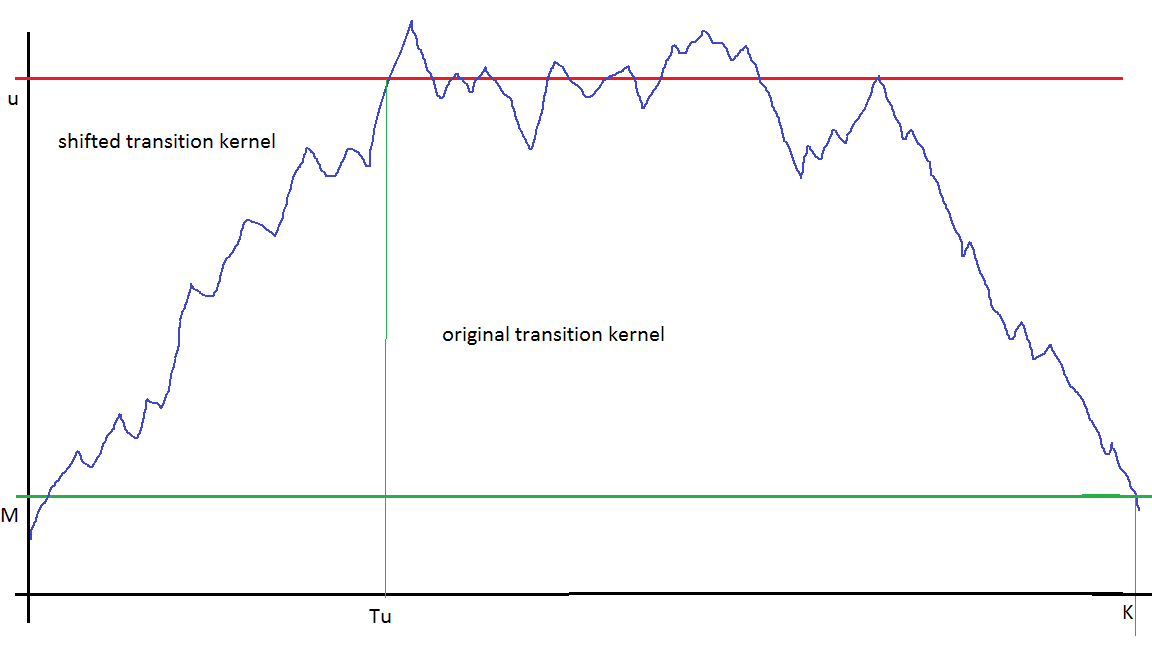
\includegraphics[width=1.0\linewidth]{pic1.png}
      \caption{\footnotesize Dual shift of Transition kernel}
      \label{fig:dual_measure}
    \end{figure}
  \end{minipage}\hfill
  \begin{minipage}[t]{0.45\linewidth}
    \begin{small}
      Algorithm:
      \begin{enumerate}
      \item Choose $\alpha$ such that $\lambda(\alpha) = 1$.
      \item draw $\sigma_0^2$ according to $\gamma$
      \item Draw $A_t$ from the shifted distribution $\tilde \nu$ for $t < T_u$, and from
        the original distribution for $t \geq T_u$.
      \item Terminate the simulation when
        $\sigma_t^2 \in \mathcal C = [0, M]$.
      \end{enumerate}
    \end{small}
  \end{minipage}
\end{frame}

\begin{frame}
  \frametitle{GARCH(p,q) processes}
  \begin{tiny}
    \begin{eqnarray*}
      %% \underbrace{
      \begin{pmatrix}
        \sigma_{t}^2 \\
        \sigma_{t-1}^2 \\
        \vdots \\
        \sigma_{t-q+2}^2 \\
        \sigma_{t-q+1}^2 \\
        X_{t-1}^2 \\
        X_{t-2}^2 \\
        \vdots \\
        X_{t-p+2}^2 \\
        X_{t-p+1}^2
      \end{pmatrix}
      %% }_{V_t}
      =
      %% \underbrace{
      \begin{pmatrix}
        \alpha_1 Z_{t-1}^2 + \beta_1 & \beta_2 & \cdots &
        \beta_{q-1} & \beta_q & \alpha_2 & \alpha_3 & \cdots & \alpha_{p-1} & \alpha_p \\
        1 & 0 & \cdots & 
        0 & 0 & 0 & 0 & \cdots & 0 & 0 \\
        \vdots & \vdots & \ddots & 
        \vdots & \vdots & \vdots & \vdots & \ddots & \vdots & \vdots \\
        0 & 0 & \cdots &
        0 & 0 & 0 & 0 & \cdots & 0 & 0 \\
        0 & 0 & \cdots &
        1 & 0 & 0 & 0 & \cdots & 0 & 0 \\
        Z_{t-1}^2 & 0 & \cdots &
        0 & 0 & 0 & 0 & \cdots & 0 & 0 \\
        0 & 0 & \cdots &
        0 & 0 & 1 & 0 & \cdots & 0 & 0 \\
        \vdots & \vdots & \ddots &
        \vdots & \vdots & \vdots & \vdots & \ddots & \vdots & \vdots \\
        0 & 0 & \cdots &
        0 & 0 & 0 & 0 & \cdots & 0 & 0 \\    
        0 & 0 & \cdots &
        0 & 0 & 0 & 0 & \cdots & 1 & 0 \\    
      \end{pmatrix}
      % }_{A_t}
      %   \underbrace{
      \begin{pmatrix}
        \sigma_{t-1}^2 \\
        \sigma_{t-2}^2 \\
        \vdots \\
        \sigma_{t-q+1}^2 \\
        \sigma_{t-q}^2 \\
        X_{t-2}^2 \\
        X_{t-3}^2 \\
        \vdots \\
        X_{t-p+1}^2 \\
        X_{t-p}^2
      \end{pmatrix} \\
      + B
      % }_{V_{t-1}} \\
    \end{eqnarray*}
  \end{tiny}
  \begin{small}
    where $B = (\omega, 0, \dots, 0)'$. Compactly
    \[
    V_t = A_t V_{t-1} + B
    \]
    By Kesten's theorem \cite{kesten:1973}:
    \[
    \lim_{u \to \infty} u^{\alpha} P(\inn{x, V_t} > u)
    = C \quad x \in \mathbb S^{d-1}
    \]
    where $d = p + q -1$ and $C$ is a constant dependent on $\alpha$.
  \end{small}
\end{frame}

\begin{frame}
  \frametitle{GARCH(p,q) processes}
  \begin{scriptsize}
    Want to simulate the rare event prob. by importance sampling
    \[
    \P(|V_t| > u) \quad u \to \infty  
    \]
    Differences from GARCH(1,1):
    \begin{itemize}
    \item Instead of $\mathcal C = [0, M]$, define
      \[
      \mathcal C = \{\vec v \in \mathbb R_+^{p+q-1}, |\vec v| \leq M\}
      \]
    \item Define the Markov random walk on the unit sphere:
      \begin{eqnarray*}
        \vec X_t &=& A_{t} \cdots A_1 \vec V_0 \over |A_{t} \cdots A_1 \vec V_0| \\
        S_t &=& \log |A_t \cdots A_1 \vec V_0| \\
        \xi_t &=& S_t - S_{t-1} =
        \log \left|A_t
          \underbrace{
            {A_{t-1} \cdots A_1 \vec V_0 \over |A_{t-1} \cdots A_1 \vec V_0|}
          }_{X_{t-1}}
        \right|
      \end{eqnarray*}
      $(\vec X_t, S_t)$ is a Markov Additive process.
    \end{itemize}
  \end{scriptsize}
\end{frame}

\begin{frame}
  \frametitle{GARCH(p,q) processes}
  As in the GARCH(1,1) case,
  \begin{eqnarray*}
    \P(|V_t| > u) &=& \pi(\mathcal C) \E_\gamma(N_u) \\
    N_u &=& \sum_{i=1}^{K-1} \1{|\vec V_t| > u}
  \end{eqnarray*}
  \begin{itemize}
  \item Knowing $\vec V_{t-1}$, $\vec V_t$ is a function of $A_t$
  \item $A_t$ is determined by $\vec X_t$, $\xi_t$ and $\vec X_{t-1}$ via
    \begin{eqnarray*}
      e^{\xi_t} \vec X_t &=& A_t \vec X_{t-1}
    \end{eqnarray*}
    Observe $A_t$ is determined by $Z_{t-1}^2$, which is given by
    \[
    Z_{t-1}^2 = {
      \inn{\vec e_{q+1}, e^{\xi_t} \vec X_{t}}
      \over
      \inn{\vec e_{1}, \vec X_{t-1}}
    }
    \]
  \end{itemize}
  \underline{$\vec V_t$ is a function of $\vec X_t$, $\xi_t$ and $\vec X_{t-1}$}
\end{frame}

\begin{frame}
  \frametitle{Importance Sampling for GARCH(p,q)}
  \begin{itemize}
  \item Define operator $T$ on a function $f \in \mathscr C_b(\mathbb
    S^{d-1}_+)$, i.e. continuous and bounded functions defined on the
    positive unit sphere.
    \[
    T_\alpha f(\vec x) = \int |A \vec x|^\alpha
    f\left({A \vec x \over |A \vec x|}\right) \P(A_t \in dA)
    \]
  \item Define right eigenfunction $r_\alpha \in \mathscr C_b(\mathbb
    S^{d-1}_+)$, and eigenvalue $\lambda(\alpha)$ by
    \[
    (T_\alpha r_\alpha)(\vec x) = \lambda(\alpha) r(\vec x)
    \]
  \item Define $Q(\vec x_{i-1}, d\vec x_{i} \times d\xi_{i})$ as the
    shifted transition kernel of $(\vec X_t, S_t)$:
    \[
    Q(\vec x_{i-1}, d\vec x_{i} \times d\xi_{i})
    =
    {e^{\alpha \xi_i} \over \lambda(\alpha) }
    {r_\alpha(\vec x_i) \over r_\alpha(\vec x_{i-1})}
    P(\vec x_{i-1}, d\vec x_{i} \times d\xi_{i})
    \]
  \end{itemize}
\end{frame}

\begin{frame}
  \frametitle{Importance Sampling for GARCH(p,q)}
  The importance sampling estimator can now be found:
    \begin{eqnarray*}
      && \E_\gamma (N_u \1{T_u < K}) \\
      &=& \E_\gamma^{\mathcal D} \left[
      N_u \1{T_u < t} e^{-\alpha S_{T_u}}
      {r_\alpha(\vec x_{0}) \over r_\alpha(\vec x_{T_u})}
    \right]
    \end{eqnarray*}
    where we have chosen $\alpha$ such that $\lambda(\alpha) = 1$.
    Note $\lambda(\alpha)$ can be identified as
    \[
    \lambda(\alpha) = \lim_{n \to \infty} (\E \|A_n \cdots A_1\|^\alpha)^{1/n}
    \]
\end{frame}

\begin{frame}
  \frametitle{The function $\log(\lambda(\alpha))$}
  \begin{minipage}{0.5\linewidth}
    \begin{small}
      \begin{itemize}
      \item 1D:
        \begin{eqnarray*}
          A &=& \alpha_1 Z^2 + \beta_1 \\
          Z &\sim& N(0,1) \\
          \lambda(\alpha) &=& \E A^\alpha          
        \end{eqnarray*}
      \item multi-dimension:
        \begin{eqnarray*}
          && \log(\lambda(\alpha)) \\
          &=&
          \lim_{n \to \infty} {1 \over n} \log \E \|A_n \cdots A_1\|^\alpha
        \end{eqnarray*}
        Estimation of $\alpha$ is trickier than in 1D.
      \end{itemize}
    \end{small}
  \end{minipage}\hfill
  \begin{minipage}{0.4\linewidth}
    \begin{figure}
      \centering
      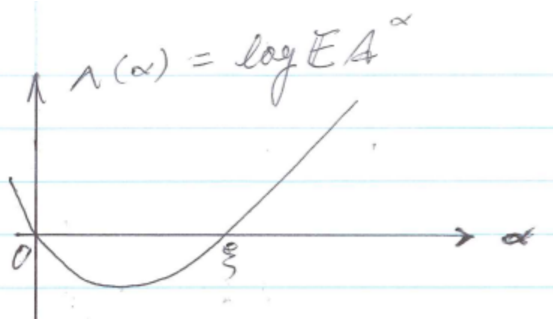
\includegraphics[width=1.0\linewidth]{pic2.pdf}
    \end{figure}
    \begin{scriptsize}
      The function $\log[\lambda(\alpha)]$ is convex and passes through the origin.
      Because $\sum_i \alpha_i + \sum_j \beta_j < 1$, it crosses the $\alpha$-axis
      under the assumption of stationarity of $\{V_n\}$.
    \end{scriptsize}
  \end{minipage}
\end{frame}

\begin{frame}
  \frametitle{Summary}
  \begin{minipage}[t]{0.4\linewidth}
    \begin{figure}
      \centering
      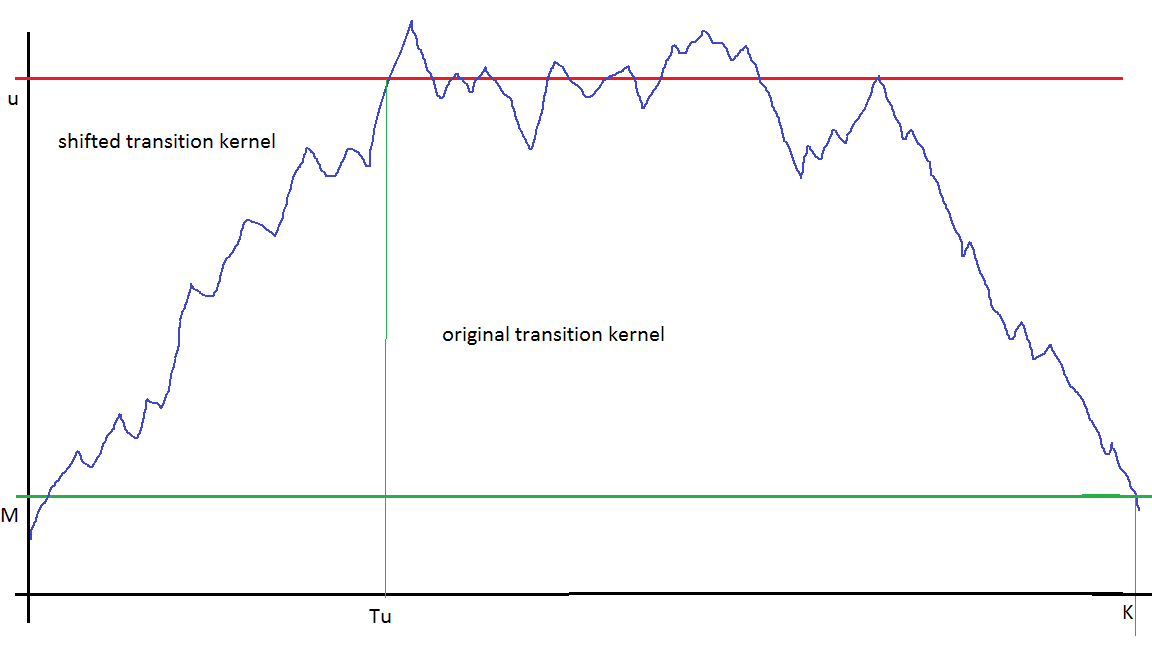
\includegraphics[width=1.0\linewidth]{pic1.png}
      \caption{\footnotesize Dual shift of Transition kernel}
    \end{figure}
  \end{minipage}\hfill
  \begin{minipage}[t]{0.6\linewidth}
    \begin{scriptsize}
      \begin{enumerate}
      \item Importance sampling estimator $\mathcal E_u$
        \[
        \P(|V| > u)
        =
        \pi(\mathcal C) \E_\gamma^{\mathcal D} \left[
          \underbrace{
            N_u e^{-\alpha S_{T_u}} {r_\alpha(\vec X_0) \over r_\alpha(\vec X_{T_u})} \1{T_u < K}
          }_{\mathcal E_u}
        \right]
        \]
      \item The estimator is consistent and efficient, i.e. it has bounded relative error:
        \[
        \sup_{u > 0} {
          \var(\mathcal E_u)
          \over
          \P(|V| > u)^2
        } < \infty
        \]
      \end{enumerate}
    \end{scriptsize}
  \end{minipage}
\end{frame}

\section{Eig. Val. of SV Smpl Cov. Mat.}
\begin{frame}
  The eigenvalues of the sample covariance matrix of a multivariate heavy-tailed 
  stochastic volatility model  
\end{frame}

\begin{frame}
  \frametitle{Motivation}
  We want to understand the eigenvalues of a sample covariance matrix
  of heavy-tailed stochastic volatility models
  $X_{i, t} = \sigma_{i, t} Z_{i,t}$ where
  \begin{itemize}
  \item $\{Z_{i,t}\}\, i,t \in \integers$: an iid. field of random variables
  \item $\{\sigma_{i,t}\}\; i,t \in \integers$: an ergodic strictly
    stationary field  of non-negative random variables.
  \item $\{Z_{i,t}\}$ and $\{\sigma_{i,t}\}$ are independent.
  \item We consider a sample of $X$, call it $\{X^n_{i, t}\}$,
    $i = 1, \dots, p$, $t = 1, \dots, n$. Define matrix
    $\{S_{i, j}\}_{i,j=1,\dots, p}$:
    \[
    S_{i,j} = \sum_{t=1}^n X^n_{i,t} X^n_{j, t}
    \]
    Write $S_i$ for $S_{i,i}$.
  \end{itemize}
\end{frame}

\begin{frame}
  \frametitle{The Model}
  \begin{scriptsize}
    \begin{minipage}[t]{0.5\linewidth}
      \textcolor[HTML]{990033}{\bf $Z$ dominates the tail}      
      \begin{itemize}
      \item $Z$ is regularly varying
        \begin{eqnarray*}
        \P(Z > x) &\sim& p_+ x^{-\alpha}, \\
        \P(Z < -x) &\sim& p_- x^{-\alpha}
        \end{eqnarray*}
        as $x \to \infty$, where $p_\pm \geq 0$ and $p_+ + p_- = 1$.
      \item $\sigma$ has lighter tails:
        $\E \sigma^{\alpha + \delta} < \infty$ for some $\delta > 0$.
      \end{itemize}
    \end{minipage}\hfill
    \begin{minipage}[t]{0.5\linewidth}
      \textcolor[HTML]{990033}{\bf $\sigma$ dominates the tail}      
      \begin{itemize}
      \item $\sigma$ is regularly varying with index $\alpha$.
        \[
        \P(\sigma > x) = x^{-\alpha} \ell(x)
        \]
        for some slowly varying function $\ell$. Moreover, we assume
        \[
        \sigma_{i, t} = \exp \left(
          \sum_{k,l \in \integers}
          \psi_{k,l} \eta_{i,k, t-l}
        \right),
        \quad
        i, t \in \integers
        \]
        where
          \begin{enumerate}
          \item {\scriptsize $\psi_{k,l} \geq 0$, $\max_{k,l} \psi_{k,l} = 1$}.
          \item {\scriptsize $\{\eta_{i,t}\}_{i, t \in \integers}$ an iid field,
            $\P(e^\eta > x) = x^{-\alpha} L(x)$, $L$ slowly varying.}
          \end{enumerate}
        % where $\{\psi_{k,l}\} \geq 0$ and $\eta_{i,t}$ is an iid field
        % satisfying $\P(e^\eta > x) = x^{-\alpha} L(x)$ for some slowly
        % varying function $L$.
      \item $\E |Z|^{\alpha + \delta} < \infty$ for some $\delta > 0$.
      \item Breiman's lemma gives
        \begin{eqnarray*}
        \P(X > x) &\sim& \E(Z_+^\alpha) \P(\sigma > x), \\
        \P(X < x) &\sim& \E(Z_-^\alpha) \P(\sigma > x)
        \end{eqnarray*}
      \end{itemize}
    \end{minipage}
\end{scriptsize}
\end{frame}

\begin{frame}
  \frametitle{Main Results: When $Z$ dominates the tail}
  \begin{scriptsize}
    \begin{theorem}
      Assume the following conditions:
      \begin{enumerate}
      \item
        $Z$ is regularly varying with index $\alpha\in (0,4) \setminus \{2\}$.
      \item
        $\{(\sigma_{it})_{t=1,2,\ldots}\}_{i=1,\ldots,p}$  is strongly
        mixing with rate function $\{\alpha_h\}$ for some $\delta>0$,
        \begin{equation}
          \label{eq:mixi}
          \sum_{h=0}^\infty \alpha_h^{\delta/(2+\delta)}<\infty\,.        
        \end{equation}
      \item
        The moment condition
        \begin{equation}
          \label{eq:moment}
          \E[\sigma^{2\max(2+\delta,\alpha+\epsilon)} ]<\infty        
        \end{equation}
        holds for the same $\delta>0$ as in \eqref{eq:mixi} and some $\epsilon>0$. 
      \end{enumerate}
      Then 
      \begin{equation}
        \label{eq:feller}
        a_n^{-2}\big(S_{1}-c_n,\ldots,S_{p}-c_n\big) \overset{d}{\to} (\xi_{1,\alpha/2},\ldots,\xi_{p,\alpha/2})\,,      
      \end{equation}
      where $\{\xi_{i,\alpha/2}\}$ are iid $\alpha/2$-stable random
      variables that are totally skewed to the right,
      \begin{equation}
        \label{eq:6:anja}
        c_n=\left\{\begin{array}{ll}
            0& \alpha \in (0,2)\,,\\
            n \,\E[X^2] &\alpha\in (2,4)\,,
          \end{array}
        \right.
      \end{equation}
      and $\{a_n\}$ satisfies $n \P(|X|>a_n)\to 1$ as $n \to 0$.
    \end{theorem}
  \end{scriptsize}
\end{frame}

\begin{frame}
  \frametitle{Main Results: When $Z$ Dominates the Tail}
  For non-diagonal elements of the sample covariance matrix, i.e.
  $S_{i,j} = \sum_{t=1}^n X_{i,t} X_{j,t}, i \neq j$, we have
  \[
  a_n^{-2} S_{i,j} \overset{P}{\to} 0
  \quad
  \text{for } i \neq j.
  \]
  where $\{a_n\}_{n\geq 1}$ is such that $n\P(|X| > a_n) \to 1$
  as $n \to \infty$. Therefore
  \begin{equation}
    a_n^{-2} \|\mtx{X X'} - \diag(\mtx{X X'}) \|
    \overset{P}{\to} 0.
  \end{equation}
  where $\|\cdot\|$ denotes the spectral norm.
\end{frame}

\begin{frame}
  \frametitle{Main Results: When $\sigma$ Dominates the Tail}
  Define
  \begin{eqnarray*}
    \psi^{i,j} &=& \max_{k,l}\{\psi_{k,l} + \psi_{k+i-j, l}\} \\
    \psi^{\vec i, \vec j}
    &=&
    \max_{1 \leq k \leq d} \psi^{i_k, j_k}
  \end{eqnarray*}
  where $\vec i = (i_1, \dots, i_d)$, $\vec j = (j_1, \dots, j_d)$.
  Note $1 \leq \psi^{i,j} \leq 2$.
  \begin{itemize}
  \item For each $i \in \integers$, the sequence
    $\{\sigma_{i,t}\}_{t \in \integers}$ is reg. var. with index $\alpha$
  \item For each $(i, j) \in \integers$, the sequence
    $\{\sigma_{i,t} \sigma_{j,t}\}_{t \in \integers}$ is
    reg. var. with index $\alpha/\psi^{i,j}$
  \item For each $(\vec i, \vec j) \in \integers^d$, the $d$-variate
    sequence
    $\{(\sigma_{i_1,t} \sigma_{j_1,t}, \dots, \sigma_{i_d,t} \sigma_{j_d,t})\}_{t \in \integers}$ is
    reg. var. with index $\alpha/\psi^{\vec i, \vec j}$.
  \end{itemize}
\end{frame}

\begin{frame}
  It follows
  \begin{itemize}
  \item For each $i \in \integers$, the sequence
    $\{X_{i,t}\}_{t \in \integers}$ is reg. var. with index $\alpha$
  \item For each $(i, j) \in \integers$, the sequence
    $\{X_{i,t} X_{j,t}\}_{t \in \integers}$ is
    reg. var. with index $\alpha/\psi^{i,j}$
  \item For each $(\vec i, \vec j) \in \integers^d$, the $d$-variate
    sequence
    $\{(X_{i_1,t} X_{j_1,t}, \dots, X_{i_d,t} X_{j_d,t})\}_{t \in \integers}$ is
    reg. var. with index $\alpha/\psi^{\vec i, \vec j}$.
  \end{itemize}
  {\bf The non-diagonal elements} of the sample covariance
    matrix (normalized by $a_n^{-2}$) may be {\bf non-zero} as
    $n \to \infty$, when $\psi^{i,j} = 2$ for some $i \neq j$.
\end{frame}

\begin{frame}
  \frametitle{Simulation Results}
  {\bf\scriptsize Eigenvalues (left) \& 1st eigenvector (right) of the sample covariance matrix}
%%  \begin{minipage}[t]{0.7\linewidth}
  \begin{figure}[htb]
    \centering
    \begin{minipage}{0.35\linewidth}
      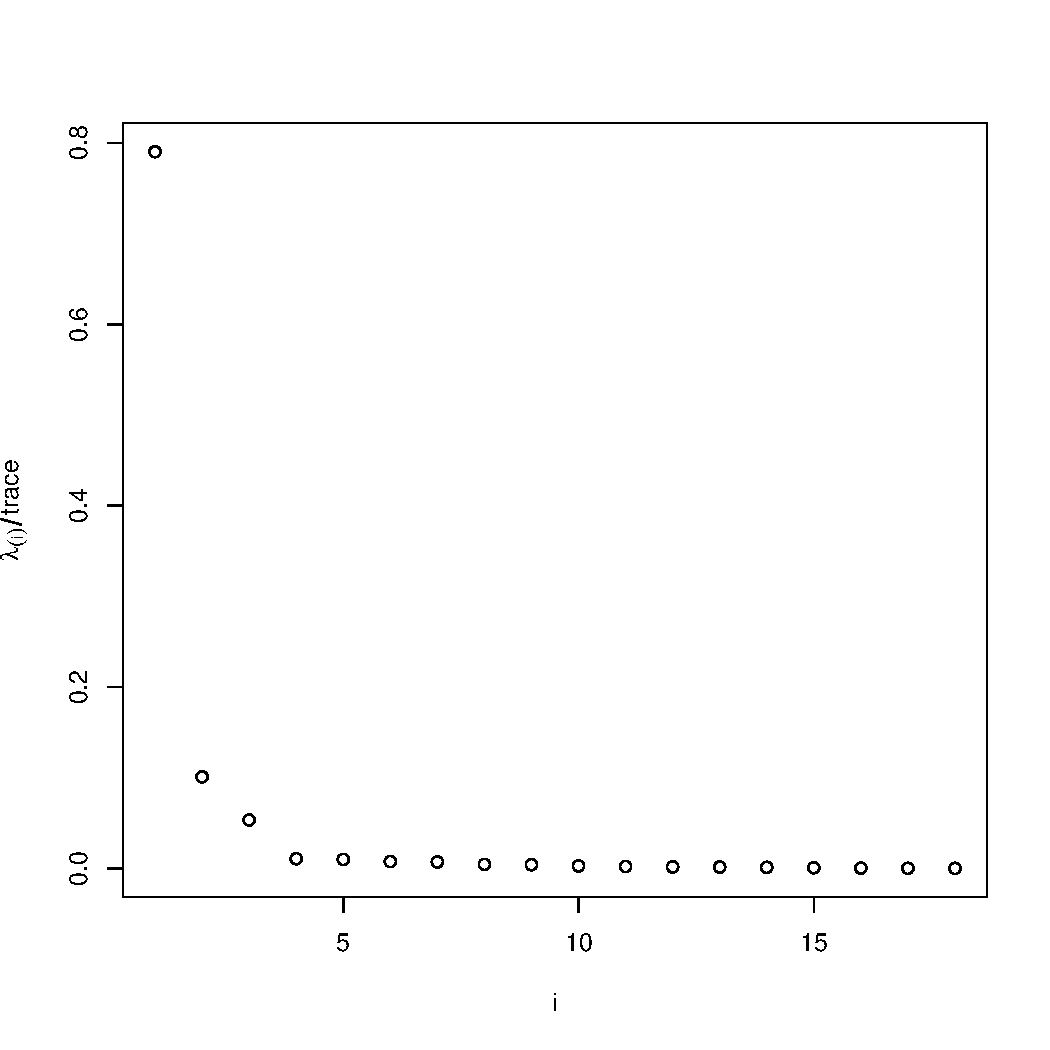
\includegraphics[width=1.0\linewidth]{HeavyTailed_eigenvalues.pdf}
    \end{minipage}\hfill
    \begin{minipage}{0.35\linewidth}
      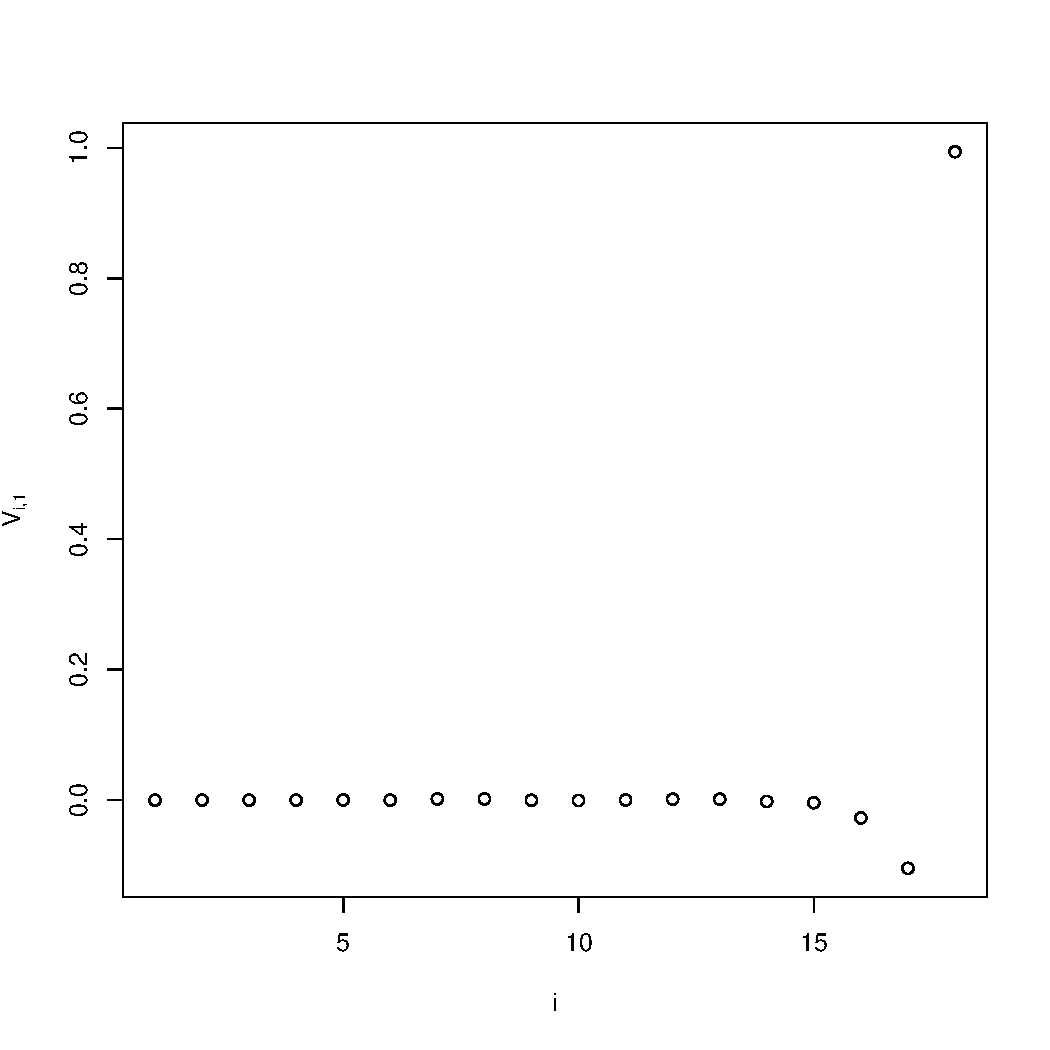
\includegraphics[width=1.0\linewidth]{HeavyTailed_eigenvector1.pdf}      
    \end{minipage}\hfill
    \begin{minipage}{0.25\linewidth}
      {\small Heavy-tailed innovation sequence}      
    \end{minipage}
    \begin{minipage}{0.35\linewidth}
      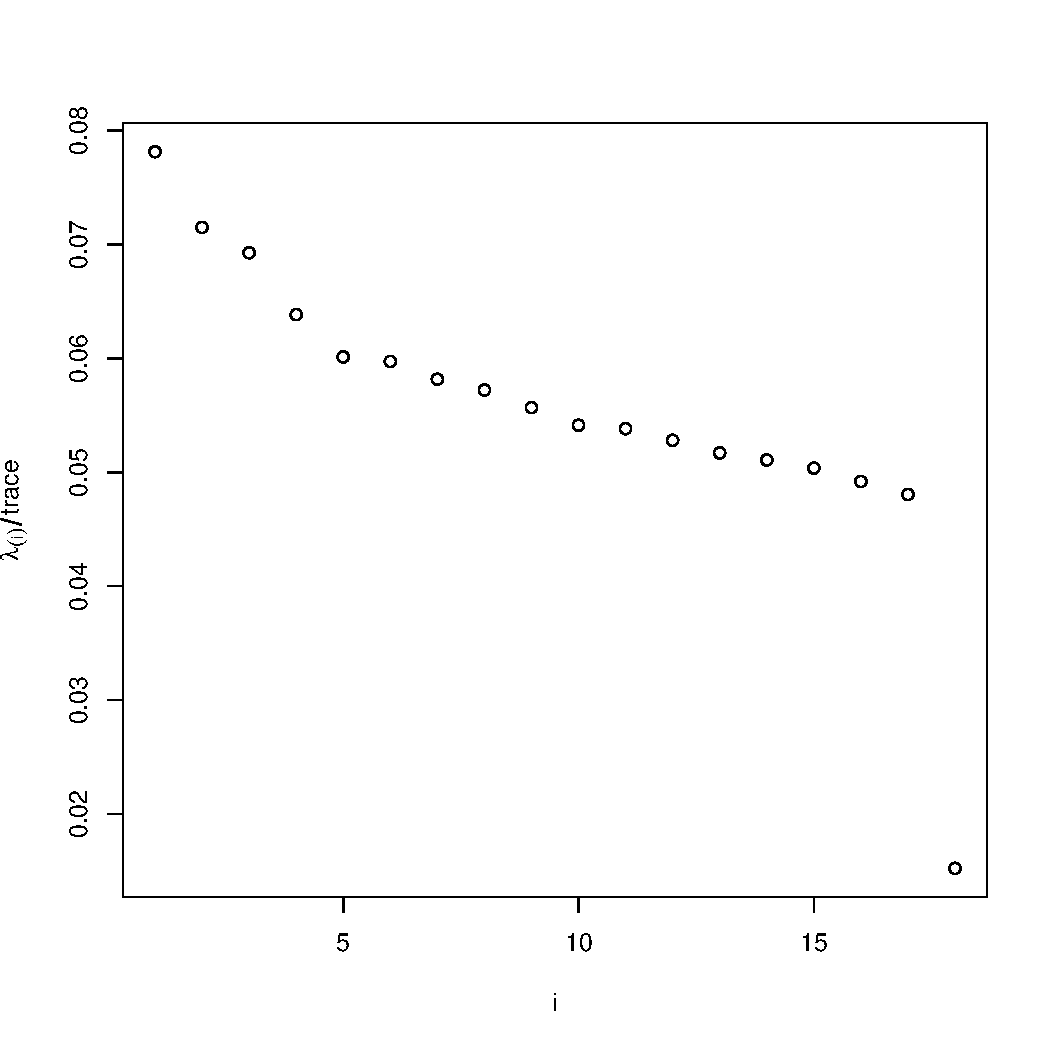
\includegraphics[width=1.0\linewidth]{LightTailedCase2_eigenvalues.pdf}
    \end{minipage}\hfill
    \begin{minipage}{0.35\linewidth}
      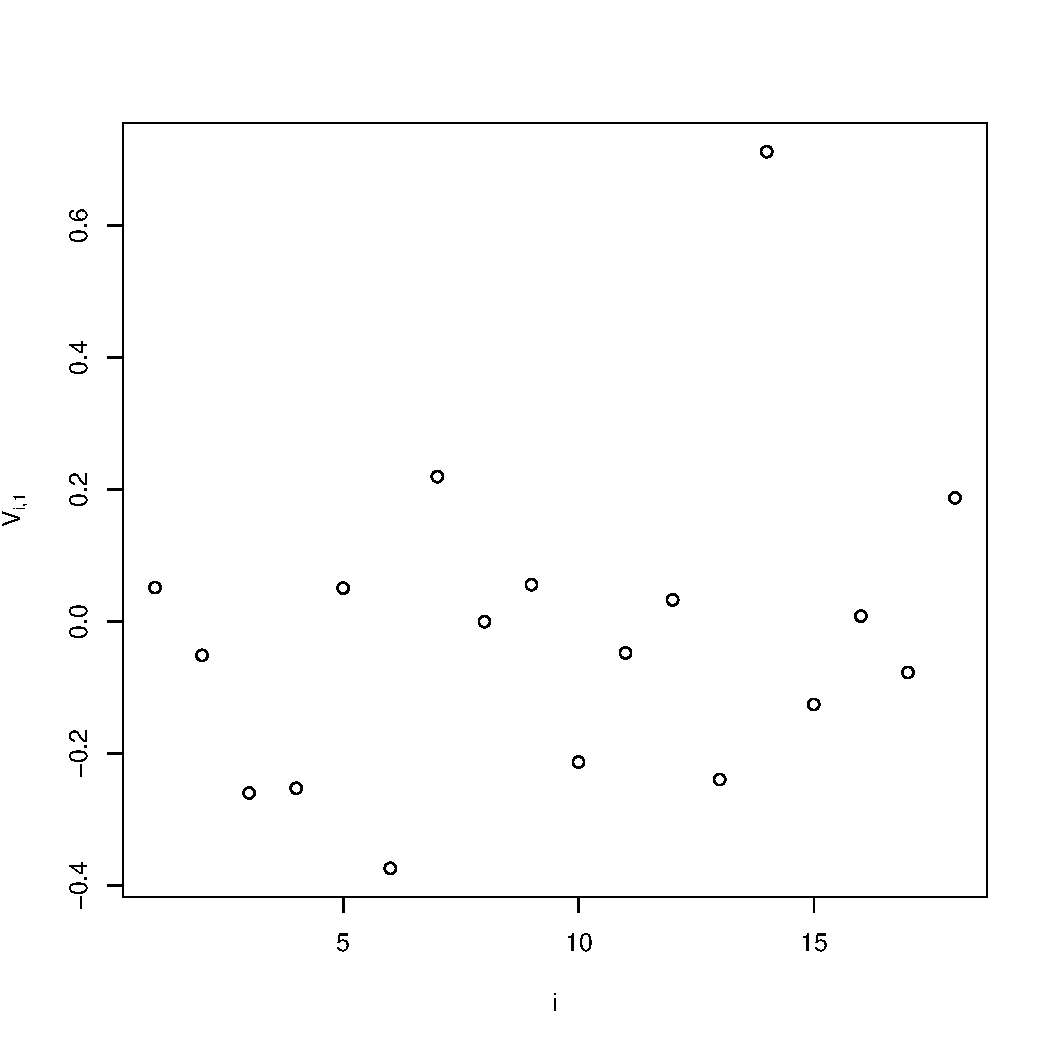
\includegraphics[width=1.0\linewidth]{LightTailedCase2_eigenvector1.pdf}
    \end{minipage}\hfill
    \begin{minipage}{0.25\linewidth}
        {\small Heavy-tailed volatility sequence with $\psi^{i,j} = 2$, for some $i, j$.}
    \end{minipage}
  \end{figure}
\end{frame}

\begin{frame}
  \frametitle{Summary}
  \begin{enumerate}
  \item Diagonal elements of the sample covariance matrix converges to $\alpha/2$-stable
    random variables.
  \item If volatility dominates the tail and a few technical conditions are satisfied, including
    the existance of $i \neq j \in \integers$ such that $\psi^{i,j} = 2$, then
    \[
    b_n^{-1} X^{n}_{i,t} X^{n}_{j,t} \overset{d}{\to} \xi_{i,j, \alpha/2}
    \]
    where $\{b_n\}_{n=1,2,\dots}$ satisfies
    $\lim_{n \to \infty} n \P(|X_{i,0} X_{j,0}| > b_n) = 1$.
    That is, the normalized non-diagonal elements do not vanish.
  \end{enumerate}
\end{frame}

\section{Eig. Val. of Smpl Cov. Mat. of Lnr. Mdl.}
\begin{frame}
  Extreme value analysis for the sample auto-covariance matrices of
  heavy-tailed multivariate time series
\end{frame}

\begin{frame}
  \frametitle{Motivation \& Approach}
  We want to understand the eigenvalues \& eigenvectors of the sample
  covariance matrix of the linear model
  \[
  X_{i,t} = \sum_{k=1}^\infty \sum_{l=1}^\infty h_{k ,l} Z_{i-k, t-l},
  \quad
  X_{i,t}^{(s)} = \sum_{k=1}^\infty \sum_{l=1}^\infty h_{k ,l} Z_{i-k, t+s-l}
  \]
  Define
  \begin{eqnarray*}
    \mtx H(s) &=& \{h_{k,l+s}\}_{k,l \in \integers} \\
    \mtx M(s) &=& \mtx H(0) \mtx H(s) \\
    \mtx X_n &=& \{X_{i,t}\}_{i=1\dots,p; t=1,\dots,n}
  \end{eqnarray*}
  Assume
  \[
  \lim_{n \to \infty} {p(n) \over n^\beta \ell(n)} = 1
  \]
  where $\ell(n)$ is some slowly-varying function and $\ell(n) \to \infty$
  if $\beta = 0$.
\end{frame}

\begin{frame}
  \frametitle{Main results: approximation of the eigenvalues}
  \begin{footnotesize}
  For $s\ge 0$:
  \begin{enumerate}
  \item We consider two disjoint cases:
    $\alpha \in (0,2)$ and $\beta\in (0,\infty)$, or
    $\alpha\in [2,4)$ and $\beta$ satisfying
    $\lim_{n \to \infty} {p(n) \over n^\beta \ell(n)} = 1$. Then
    \begin{equation*}
      a_{np}^{-2} \max_{i=1,\ldots,p}
      |\lambda_{(i)}(s)-\delta_{(i)}(s)|
      \overset{P}{\to} 0,
      \quad
      n \to \infty.
    \end{equation*}
  \item
    Assume $\beta\in [0,1]$.
    If $\alpha \in (0,2]$, $\E[Z^2]=\infty$ or $\alpha\in [2,4)$, $\E [Z^2]<\infty$ and $\beta\in (\alpha/2-1,1]$ then
    \begin{equation*}
    a_{np}^{-2} \max_{i=1,\ldots,p} |\lambda_{(i)}(s)-\gamma_{(i)}^\rightarrow(s)| \overset{P}{\to} 0, \quad n \to \infty.
    \end{equation*}
    Assume $\beta>1$. If $\alpha \in (0,2]$, $\E[Z^2]=\infty$ or $\alpha\in [2,4)$, $\E [Z^2]<\infty$ and $\beta^{-1}\in(\alpha/2-1,1]$. Then
      \begin{equation*}
      a_{np}^{-2} \max_{i=1,\ldots,p} |\lambda_{(i)}(s)-\gamma_{(i)}^\downarrow(s)| \overset{P}{\to} 0, \quad n \to \infty.
      \end{equation*}
  \end{enumerate}
  \end{footnotesize}
\end{frame}

\begin{frame}
  \frametitle{Main results: approximation of the eigenvalues}
  \begin{footnotesize}
    Notations:
    \begin{itemize}
    \item $\delta_{(i)}(s)$: $i$-th upper order statistic of
      \[
      \big\{Z_{(i),np}^2 v_j(s)\,, i=1,\ldots,p\,;j=1,2,\ldots\big\}
      \]
    \item $\gamma_{(i)}^\rightarrow(s)$: $i$-th upper order statistic
      of
      \[
      \big\{D_{i}^\rightarrow v_j(s), i=1,\ldots,p\,;j=1,2,\ldots\big\}
      \]
    \item $\gamma_{(1)}^\downarrow(s)$: $i$-th upper order statistic
      of
      \[
      \big\{D_{t}^\downarrow v_j(s), t=1,\ldots,n\,;j=1,2,\ldots\big\}
      \]
    \end{itemize}
    where
    \begin{itemize}
    \item $v_1(s) > v_2(s) > \cdots$ are singular values
      of $\mtx M(s)$.
    \item
      \begin{equation*}
        D_i^\rightarrow=D_i^{(n),\rightarrow}=\sum_{t=1}^n Z_{it}^2\,, \qquad
        i=1,\ldots,p;\quad  n=1,2,\ldots\,,
      \end{equation*}
      \begin{equation*}
        D_t^\downarrow=D_t^{(n),\downarrow}= \sum_{i=1}^p
        Z_{it}^2\,,\qquad
        t=1,\ldots,n;\; \quad p=1,2,\ldots\,,
      \end{equation*}
    \end{itemize}
  \end{footnotesize}
\end{frame}

\begin{frame}
  \frametitle{Main results: point process convergence}
  \begin{small}
    \begin{theorem}
      Define
      \begin{equation*}
        N_n^{\lambda,s}=\sum_{i=1}^p \varepsilon_{a_{np}^{-2}(\lambda_{(i)}(0),\ldots,\lambda_{(i)}(s))} \,.
      \end{equation*}
      $N_n^{\lambda,s}$ converge weakly in the space of point measures
      with state space $(0,\infty)^{s+1}$ equipped with the vague topology.
      \begin{equation*}
        N_n^{\lambda,s} \overset{d}{\to} N= \sum_{i=1}^\infty
        \sum_{j=1}^{\infty} \varepsilon_{\Gamma_i^{-2/\alpha}
          (v_j(0),\ldots,v_j(s))}, \qquad n \to \infty.
      \end{equation*}
      where $\Gamma_i = \sum_{k=1}^i E_k, E_k \sim
      \text{Exp}(1)$. $\{E_i\}_{i=1,2,\dots}$ is an iid sequence. 
    \end{theorem}
  \end{small}
\end{frame}

\begin{frame}
  \frametitle{Main Results: Assumptions}
  Assume
  \begin{scriptsize}
    \begin{enumerate}
    \item Regular variation of $Z$:
      \begin{equation*}
        \P(Z>x)\sim p_+ \dfrac{L(x)}{x^{\alpha}}\quad\mbox{and}\quad  \P(Z\le -x)\sim p_-
        \dfrac{L(x)}{x^{\alpha}}\,,\qquad x \to \infty,
      \end{equation*}
      for some tail index $\alpha \in (0, 4)$, constants $p_+,p_-\ge 0$ with
      $p_++p_-=1$ and a slowly varying function $L$.
    \item Either $\alpha \in (0,2]$, $\E[Z^2]=\infty$ and $\beta \ge 0$,
      or $\alpha \in [2,4)$, $\E[Z^2]<\infty$ and
      $\lim_{n \to \infty} {p(n) \over n^\beta \ell(n)} = 1$.
    \item $\E[Z]=0$ whenever $\E |Z| <\infty$.
    \item Summability of $\{h_{k,l}\}$
      \begin{equation*}
        \sum_{l \in \integers} \sum_{k\in \integers} |h_{kl}|^{\delta} <\infty
      \end{equation*}
      for some $\delta\in (0,\min({\alpha/2},1))$
    \end{enumerate}
  \end{scriptsize}
\end{frame}

\begin{frame}
  \frametitle{ }
  \begin{centering}
    \Large Thank you for your attention!
  \end{centering}
 \end{frame}

\bibliographystyle{unsrt}
\bibliography{../../thesis/econophysics}
\end{document} 
